% ============================================================
% 基于TCGA多组学数据挖掘的乳腺癌分子特征综合分析
% 格式：中国高校本科毕业论文
% ============================================================
\documentclass[12pt,a4paper]{article}

% ---- 中文支持 ----
\usepackage[UTF8, heading=true]{ctex}
\ctexset{
  section/format = \Large\bfseries\centering,
  subsection/format = \large\bfseries,
  subsubsection/format = \normalsize\bfseries,
}

% ---- 页面 ----
\usepackage[top=2.5cm, bottom=2.5cm, left=2.5cm, right=2.5cm]{geometry}
\usepackage{setspace}
\onehalfspacing

% ---- 字体：全部宋体 ----
\setmainfont{SimSun}[AutoFakeBold=2.5]
\setsansfont{SimSun}
\setmonofont{SimSun}[Scale=0.9]

% ---- 图表 ----
\usepackage{graphicx}
\usepackage{float}
\usepackage{booktabs}
\usepackage{multirow}
\usepackage{caption}
\captionsetup{font={small,bf}, labelsep=space, justification=centering}

% ---- 数学 ----
\usepackage{amsmath}

% ---- 代码框：黑色字体，灰底 ----
\usepackage{listings}
\usepackage{xcolor}
\lstset{
  language=R,
  basicstyle=\small\ttfamily,
  keywordstyle=\bfseries,
  commentstyle=\itshape,
  stringstyle=,
  numbers=left,
  numberstyle=\tiny,
  numbersep=8pt,
  frame=single,
  framesep=5pt,
  rulecolor=\color{black},
  backgroundcolor=\color{black!3},
  breaklines=true,
  breakatwhitespace=false,
  showstringspaces=false,
  tabsize=2,
  captionpos=b,
  aboveskip=10pt,
  belowskip=8pt,
  extendedchars=false,
  literate={-}{-}1,
}

% ---- 引用 ----
\usepackage[numbers,sort&compress]{natbib}

% ---- 超链接 ----
\usepackage[colorlinks=false]{hyperref}

% ---- 页眉页脚 ----
\usepackage{fancyhdr}
\pagestyle{fancy}
\fancyhf{}
\fancyhead[C]{\small 基于TCGA多组学数据挖掘的乳腺癌分子特征综合分析}
\fancyfoot[C]{\thepage}
\renewcommand{\headrulewidth}{0.4pt}

% ---- 标题 ----
\title{\LARGE\textbf{基于TCGA多组学数据挖掘的乳腺癌分子特征综合分析}}
\author{\Large 《生物大数据分析》期末报告}
\date{2026年5月}

\begin{document}

\maketitle
\thispagestyle{empty}

% ===== 摘要 =====
\begin{center}
\textbf{摘\quad 要}
\end{center}

乳腺癌是全球发病率最高的恶性肿瘤之一，其高度的分子异质性为精准诊疗带来了巨大挑战。本研究基于TCGA-BRCA数据集（1,105例肿瘤 + 113例正常组织，25,981个基因），运用DESeq2差异表达分析、Random Forest/LASSO分类、K-means聚类、WGCNA共表达网络、Cox生存分析等数据挖掘方法，系统分析乳腺癌分子特征。共鉴定6,768个差异表达基因（上调4,334，下调2,434）；Random Forest和LASSO分类准确率均为75.8\%；PCA分析显示PC1=15.3\%，K-means最优聚类数K=2；WGCNA识别9个共表达模块，枢纽基因模块隶属度达0.959；多变量Cox回归C-index=0.767，Stage IV风险比达29.82。

\vspace{0.5em}
\noindent\textbf{关键词：}乳腺癌；TCGA；数据挖掘；差异表达分析；WGCNA；机器学习分类；生存分析；R语言

\newpage
\tableofcontents
\newpage

% ===== 1 引言 =====
\section{引言}

\subsection{研究背景}

据国际癌症研究机构（IARC）GLOBOCAN 2022统计，全球每年新发癌症约2,000万例，死亡约970万例\cite{sung2024}。女性乳腺癌以约230万例新发病例居全球恶性肿瘤发病率首位，同年导致约67万例死亡。在中国，乳腺癌发病率和死亡率持续上升，且发病年龄显著低于欧美国家，构成重大的公共卫生负担。

乳腺癌的发生发展涉及多基因突变累积、表观遗传重塑及信号通路交互失调等复杂分子过程\cite{hanahan2011}。高通量测序技术的普及使大规模癌症基因组数据的积累成为可能。以癌症基因组图谱（The Cancer Genome Atlas, TCGA）为代表的国际合作项目，为研究者提供了涵盖基因组、转录组、表观基因组及蛋白质组的海量公开数据资源\cite{tcga2012}。

\subsection{乳腺癌分子分型}

Perou等\cite{perou2000}于2000年首次基于基因表达谱提出分子分型体系。当前国际广泛认可的固有分子亚型包括：（1）Luminal A型（约占50\%--60\%），特征为ER阳性、HER2阴性；（2）Luminal B型（约占15\%--20\%）；（3）HER2过表达型（约占10\%--15\%）；（4）三阴性/Basal-like型（约占15\%--20\%），侵袭性最强。

\subsection{研究内容与论文结构}

本研究以TCGA-BRCA数据为对象，综合运用差异表达分析、机器学习分类、聚类分析、WGCNA共表达网络和生存分析等方法，系统开展乳腺癌分子特征挖掘。论文结构：第2章材料与方法；第3章结果；第4章讨论；第5章结论。

% ===== 2 材料与方法 =====
\section{材料与方法}

\subsection{数据来源}

本研究数据来自TCGA-BRCA项目，包含mRNA转录组数据（HiSeq RNA-seq, STAR-Counts流程）和临床注释数据。TCGA样本条形码采用标准化分层命名规则，前12个字符为患者级唯一标识符，样本类型代码（第14--15位）中01表示原发实体瘤，11表示癌旁正常组织。

\subsection{数据预处理}

\subsubsection{样本分类与基因过滤}

解析TCGA条形码区分肿瘤与正常样本。采用独立过滤策略，保留至少在10\%肿瘤样本中counts$\geq$10的基因（参考DESeq2推荐准则）。

\subsubsection{基因标识符映射与TPM标准化}

通过org.Hs.eg.db注释包将Ensembl Gene ID映射为标准Gene Symbol，对一对多映射保留平均表达量最高的条目。采用Transcripts Per Million（TPM）进行归一化：

\begin{equation}
TPM_i = \frac{Counts_i / (GeneLength_i / 1000)}{\sum_j [Counts_j / (GeneLength_j / 1000)]} \times 10^6
\end{equation}

\subsubsection{临床数据清洗}

从原始临床变量中提取年龄、病理分期、ER/PR/HER2状态等核心变量。分子亚型按ER/PR/HER2免疫组化状态分类。缺失值采用中位数（数值型）或众数（分类型）填补。最终将表达矩阵与临床数据以患者ID为锚点进行对齐，匹配1,105例患者。

\subsection{数据挖掘算法}

\subsubsection{差异表达分析}

采用DESeq2\cite{love2014}进行肿瘤组织（n=1,105）与正常组织（n=113）的差异表达分析。DESeq2基于负二项分布对RNA-seq计数数据建模，通过经验贝叶斯收缩改进离散度估计的稳定性，使用Wald检验评估组间差异的显著性。显著性阈值取FDR$<0.05$（Benjamini-Hochberg校正）且$|\log_2\text{FC}|>1$。功能富集分析采用g:Profiler\cite{kolberg2023}，覆盖GO、KEGG和Reactome数据库。

\subsubsection{机器学习分类}

比较Random Forest（ntree=500）\cite{breiman2001}和LASSO多分类回归（family=``multinomial'', $\alpha=1$, 5折交叉验证）\cite{friedman2010}的分类性能。输入特征为Top 500可变基因的$\log_2(\text{TPM}+1)$表达矩阵。训练集与测试集按7:3分层划分（set.seed=42）。评估指标包括准确率（Accuracy）、Kappa系数和Macro F1分数。

\subsubsection{聚类分析}

综合运用PCA（Top 2000可变基因）、t-SNE（perplexity=30, max\_iter=1000）、K-means（K=2至10评估轮廓系数）和层次聚类（Ward.D2方法，Pearson相关系数距离）。

\subsubsection{WGCNA共表达网络分析}

WGCNA\cite{langfelder2008}使用Top 5000可变基因的$\log_2(\text{TPM}+1)$矩阵。分析流程：（1）计算基因间Pearson相关系数构建相似性矩阵；（2）选择软阈值幂函数（scale-free $R^2>0.8$）构建邻接矩阵；（3）构建拓扑重叠矩阵（TOM）；（4）动态树切割识别模块（minModuleSize=30, mergeCutHeight=0.25）；（5）计算模块特征基因与临床性状的相关性；（6）通过模块内连接度（Module Membership, MM）识别枢纽基因。

\subsubsection{生存分析}

采用Kaplan-Meier生存曲线（log-rank检验）和Cox比例风险回归\cite{therneau2000}评估临床及分子特征的预后价值。Cox模型纳入年龄、病理分期和分子亚型。此外，采用LASSO-Cox\cite{simon2011}方法构建预后基因标记，按中位风险得分将患者分为高风险组和低风险组。

\subsection{分析环境}

R 4.6.0 + Bioconductor 3.23，Windows 11环境。主要R包：DESeq2、caret、randomForest、glmnet、WGCNA、survival、survminer、gprofiler2、pheatmap、ggplot2。

% ===== 3 结果 =====
\section{结果}

\subsection{数据预处理结果}

原始表达矩阵包含60,660个基因，经低表达过滤后保留25,981个（42.8\%）。肿瘤样本1,105例，正常组织113例。临床数据匹配后获得1,105例患者，分子亚型分布为：Luminal A 827例、Luminal B 126例、HER2-enriched 37例、Triple Negative 115例。病理分期：Stage I 183例、II 651例、III 251例、IV 20例。生存信息：死亡事件87例，存活1,018例。

\begin{table}[H]
\centering
\caption{数据概览}
\begin{tabular}{ll}
\toprule
指标 & 数值 \\
\midrule
过滤后基因数 & 25,981 \\
肿瘤样本 & 1,105 \\
正常样本 & 113 \\
临床变量 & 21 \\
死亡事件/存活 & 87 / 1,018 \\
\bottomrule
\end{tabular}
\end{table}

\begin{figure}[H]
\centering
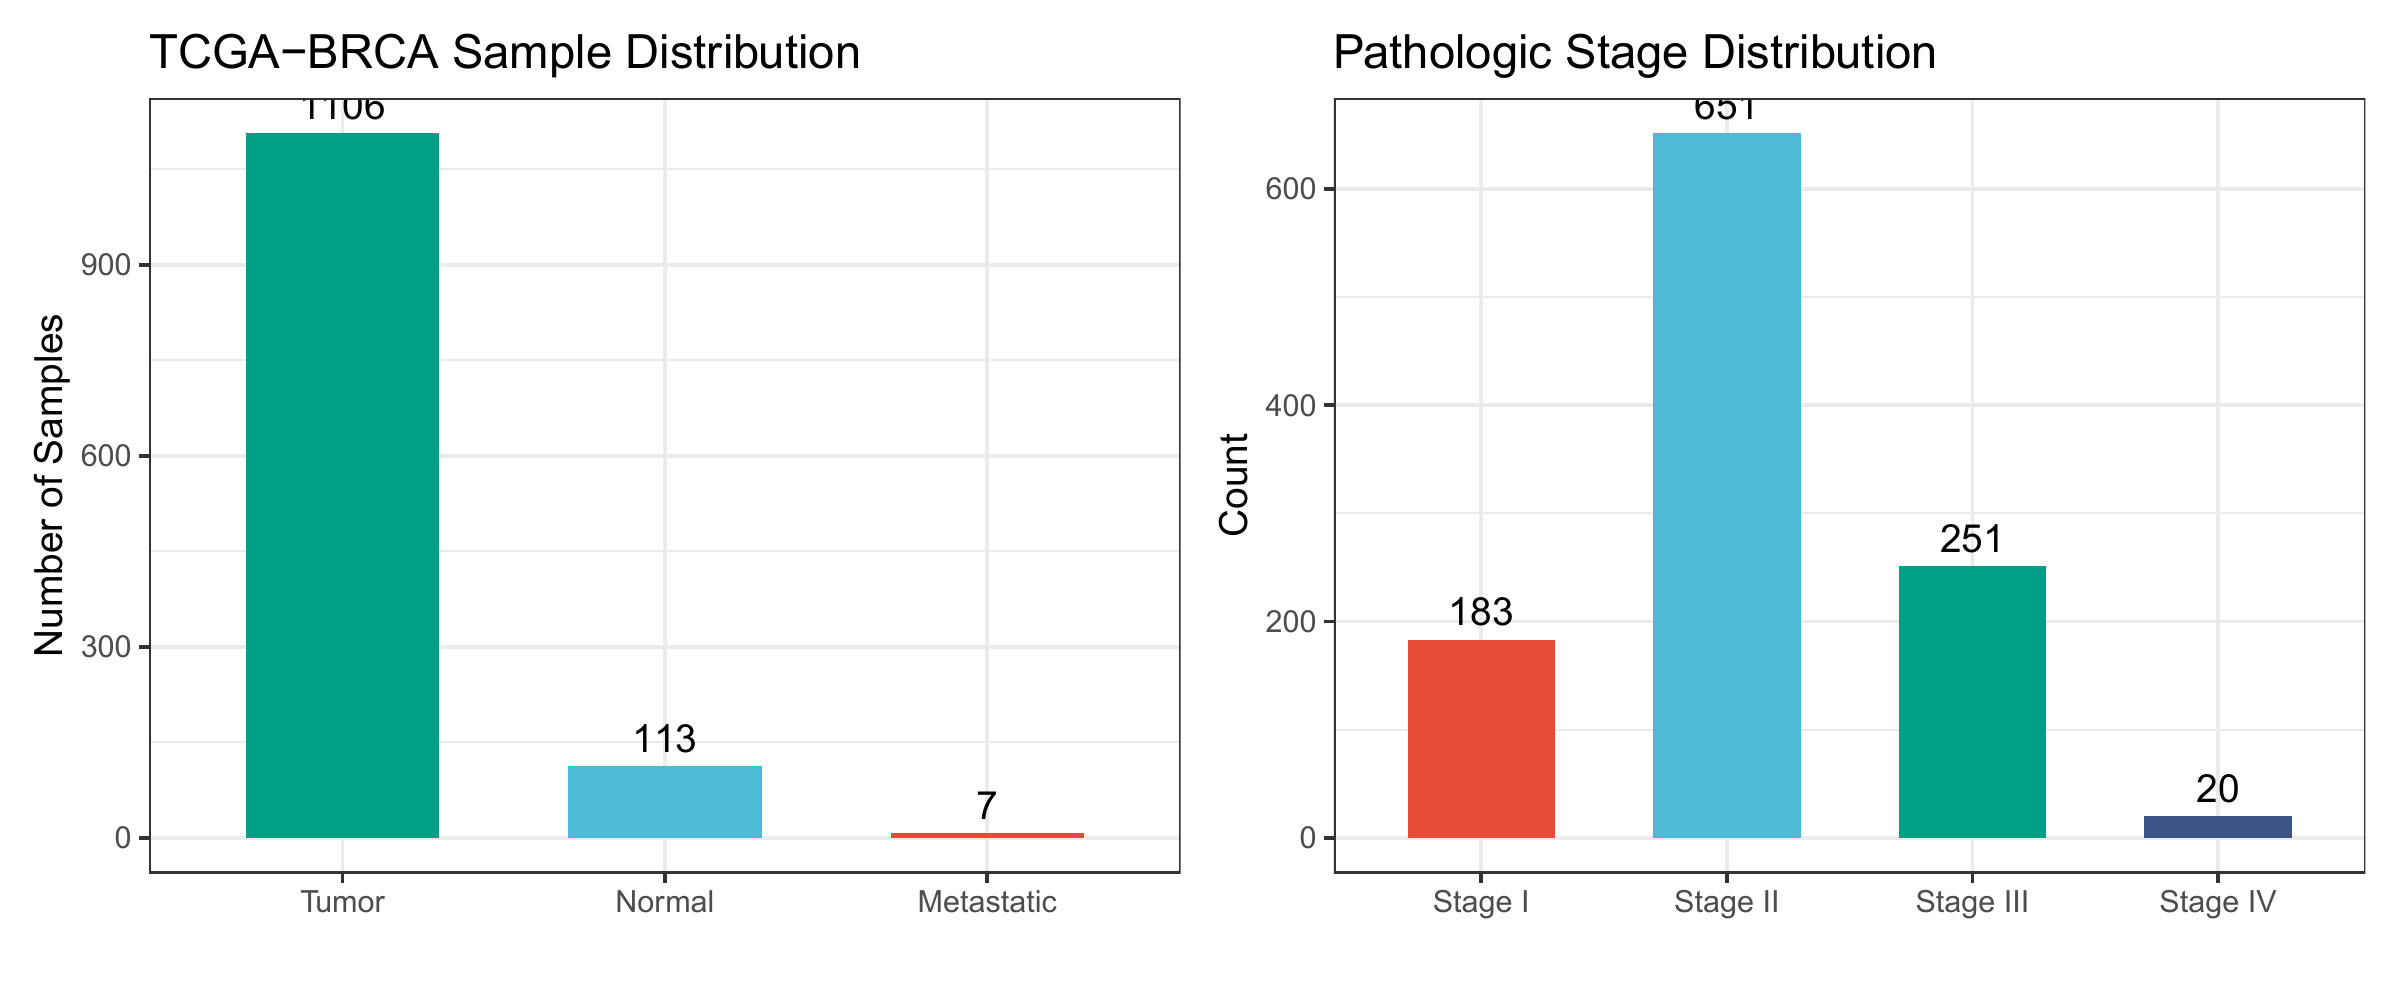
\includegraphics[width=0.85\textwidth]{figures/fig1_sample_overview.png}
\caption{TCGA-BRCA样本分布与病理分期分布}
\end{figure}

\subsection{差异表达分析}

DESeq2共鉴定6,768个显著差异表达基因（$|\log_2\text{FC}|>1$, padj$<0.05$），其中上调4,334个，下调2,434个。上调基因数量约为下调的1.78倍，提示肿瘤组织中转录激活事件多于转录抑制事件。

\begin{figure}[H]
\centering
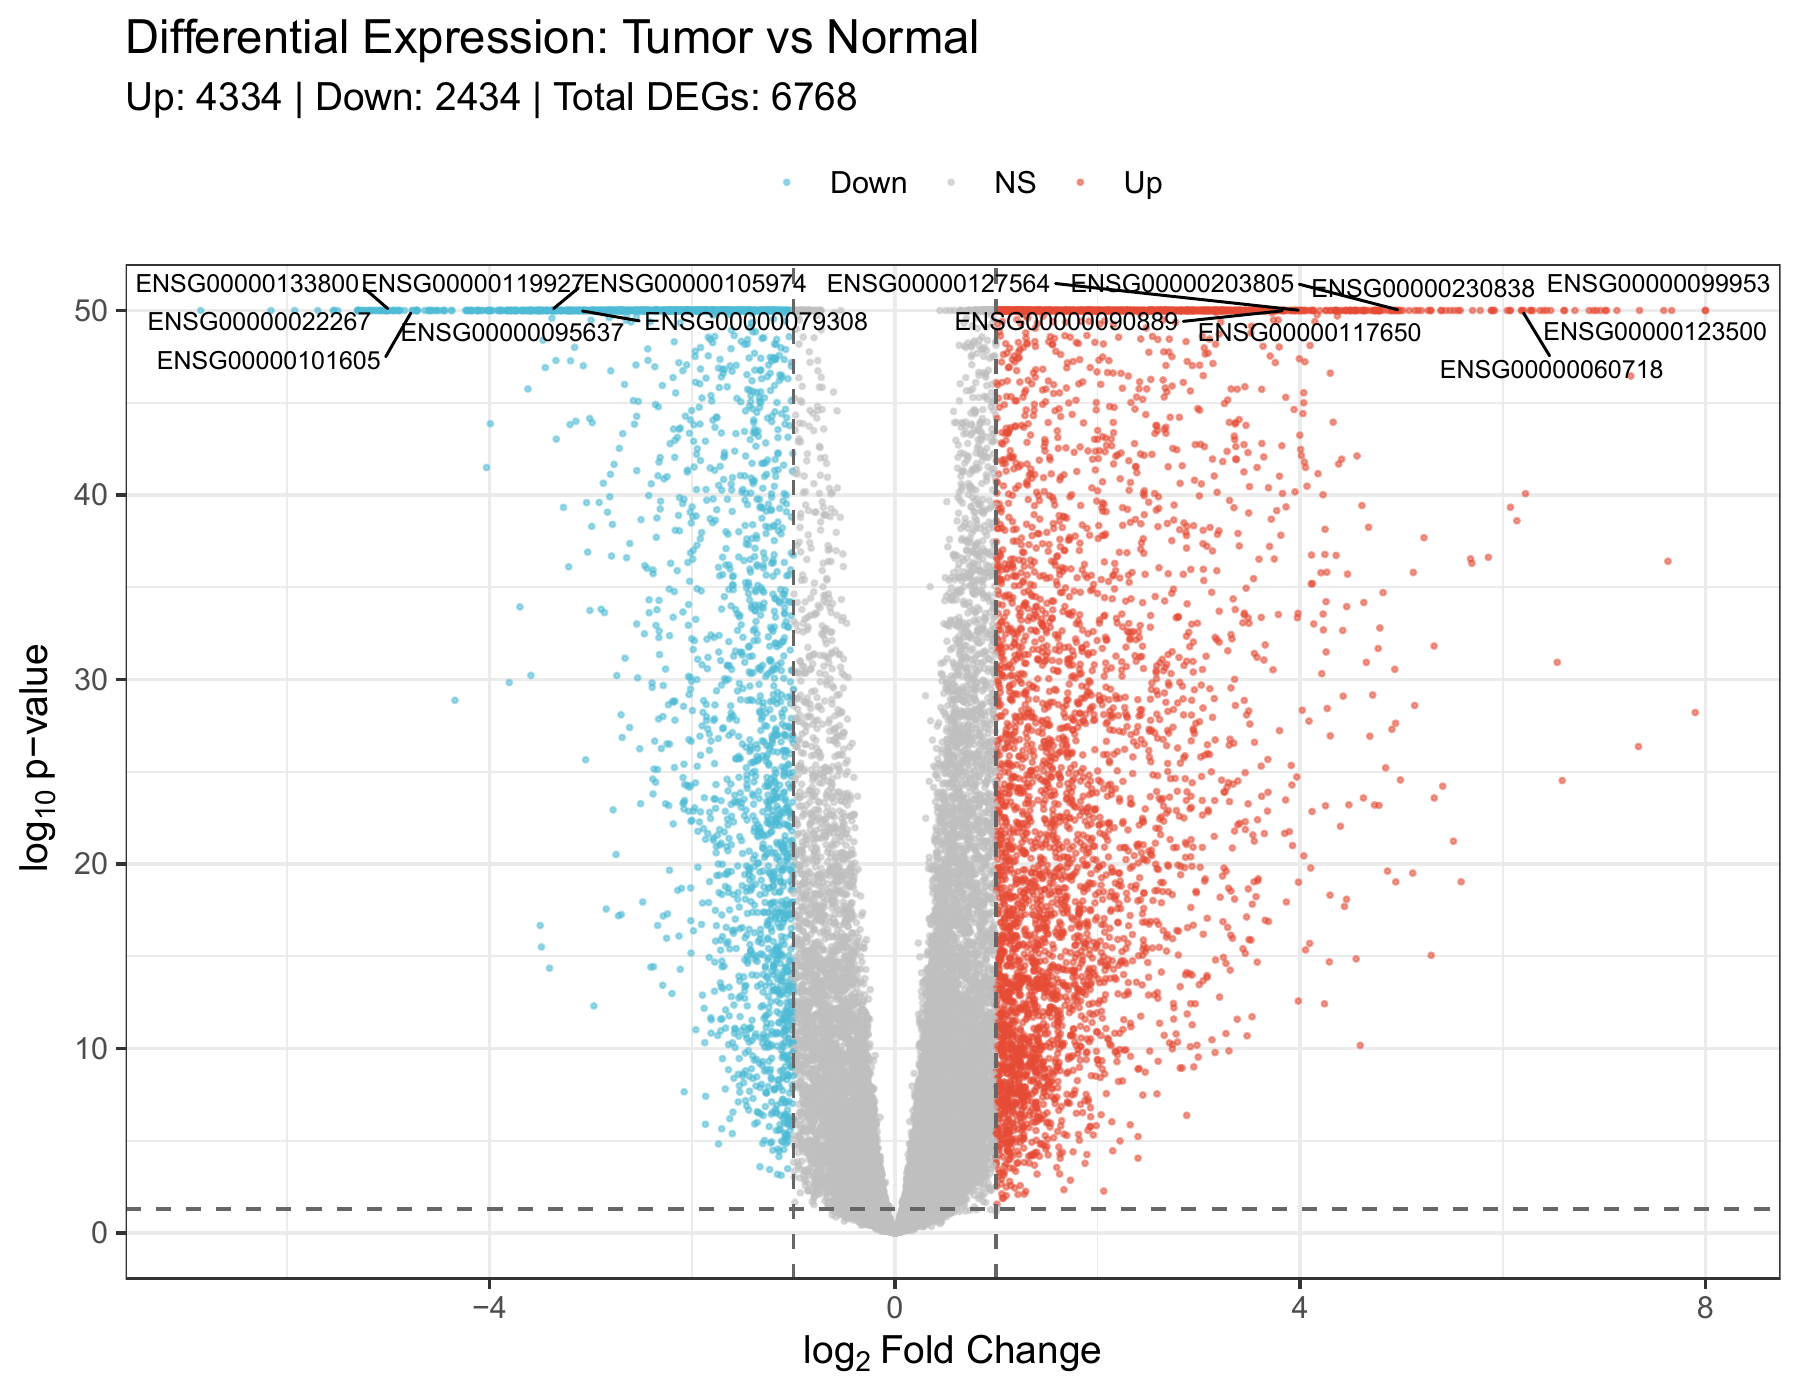
\includegraphics[width=0.85\textwidth]{figures/fig2_volcano_enhanced.png}
\caption{差异表达火山图。红色：上调基因；蓝色：下调基因；灰色：不显著}
\end{figure}

\begin{figure}[H]
\centering
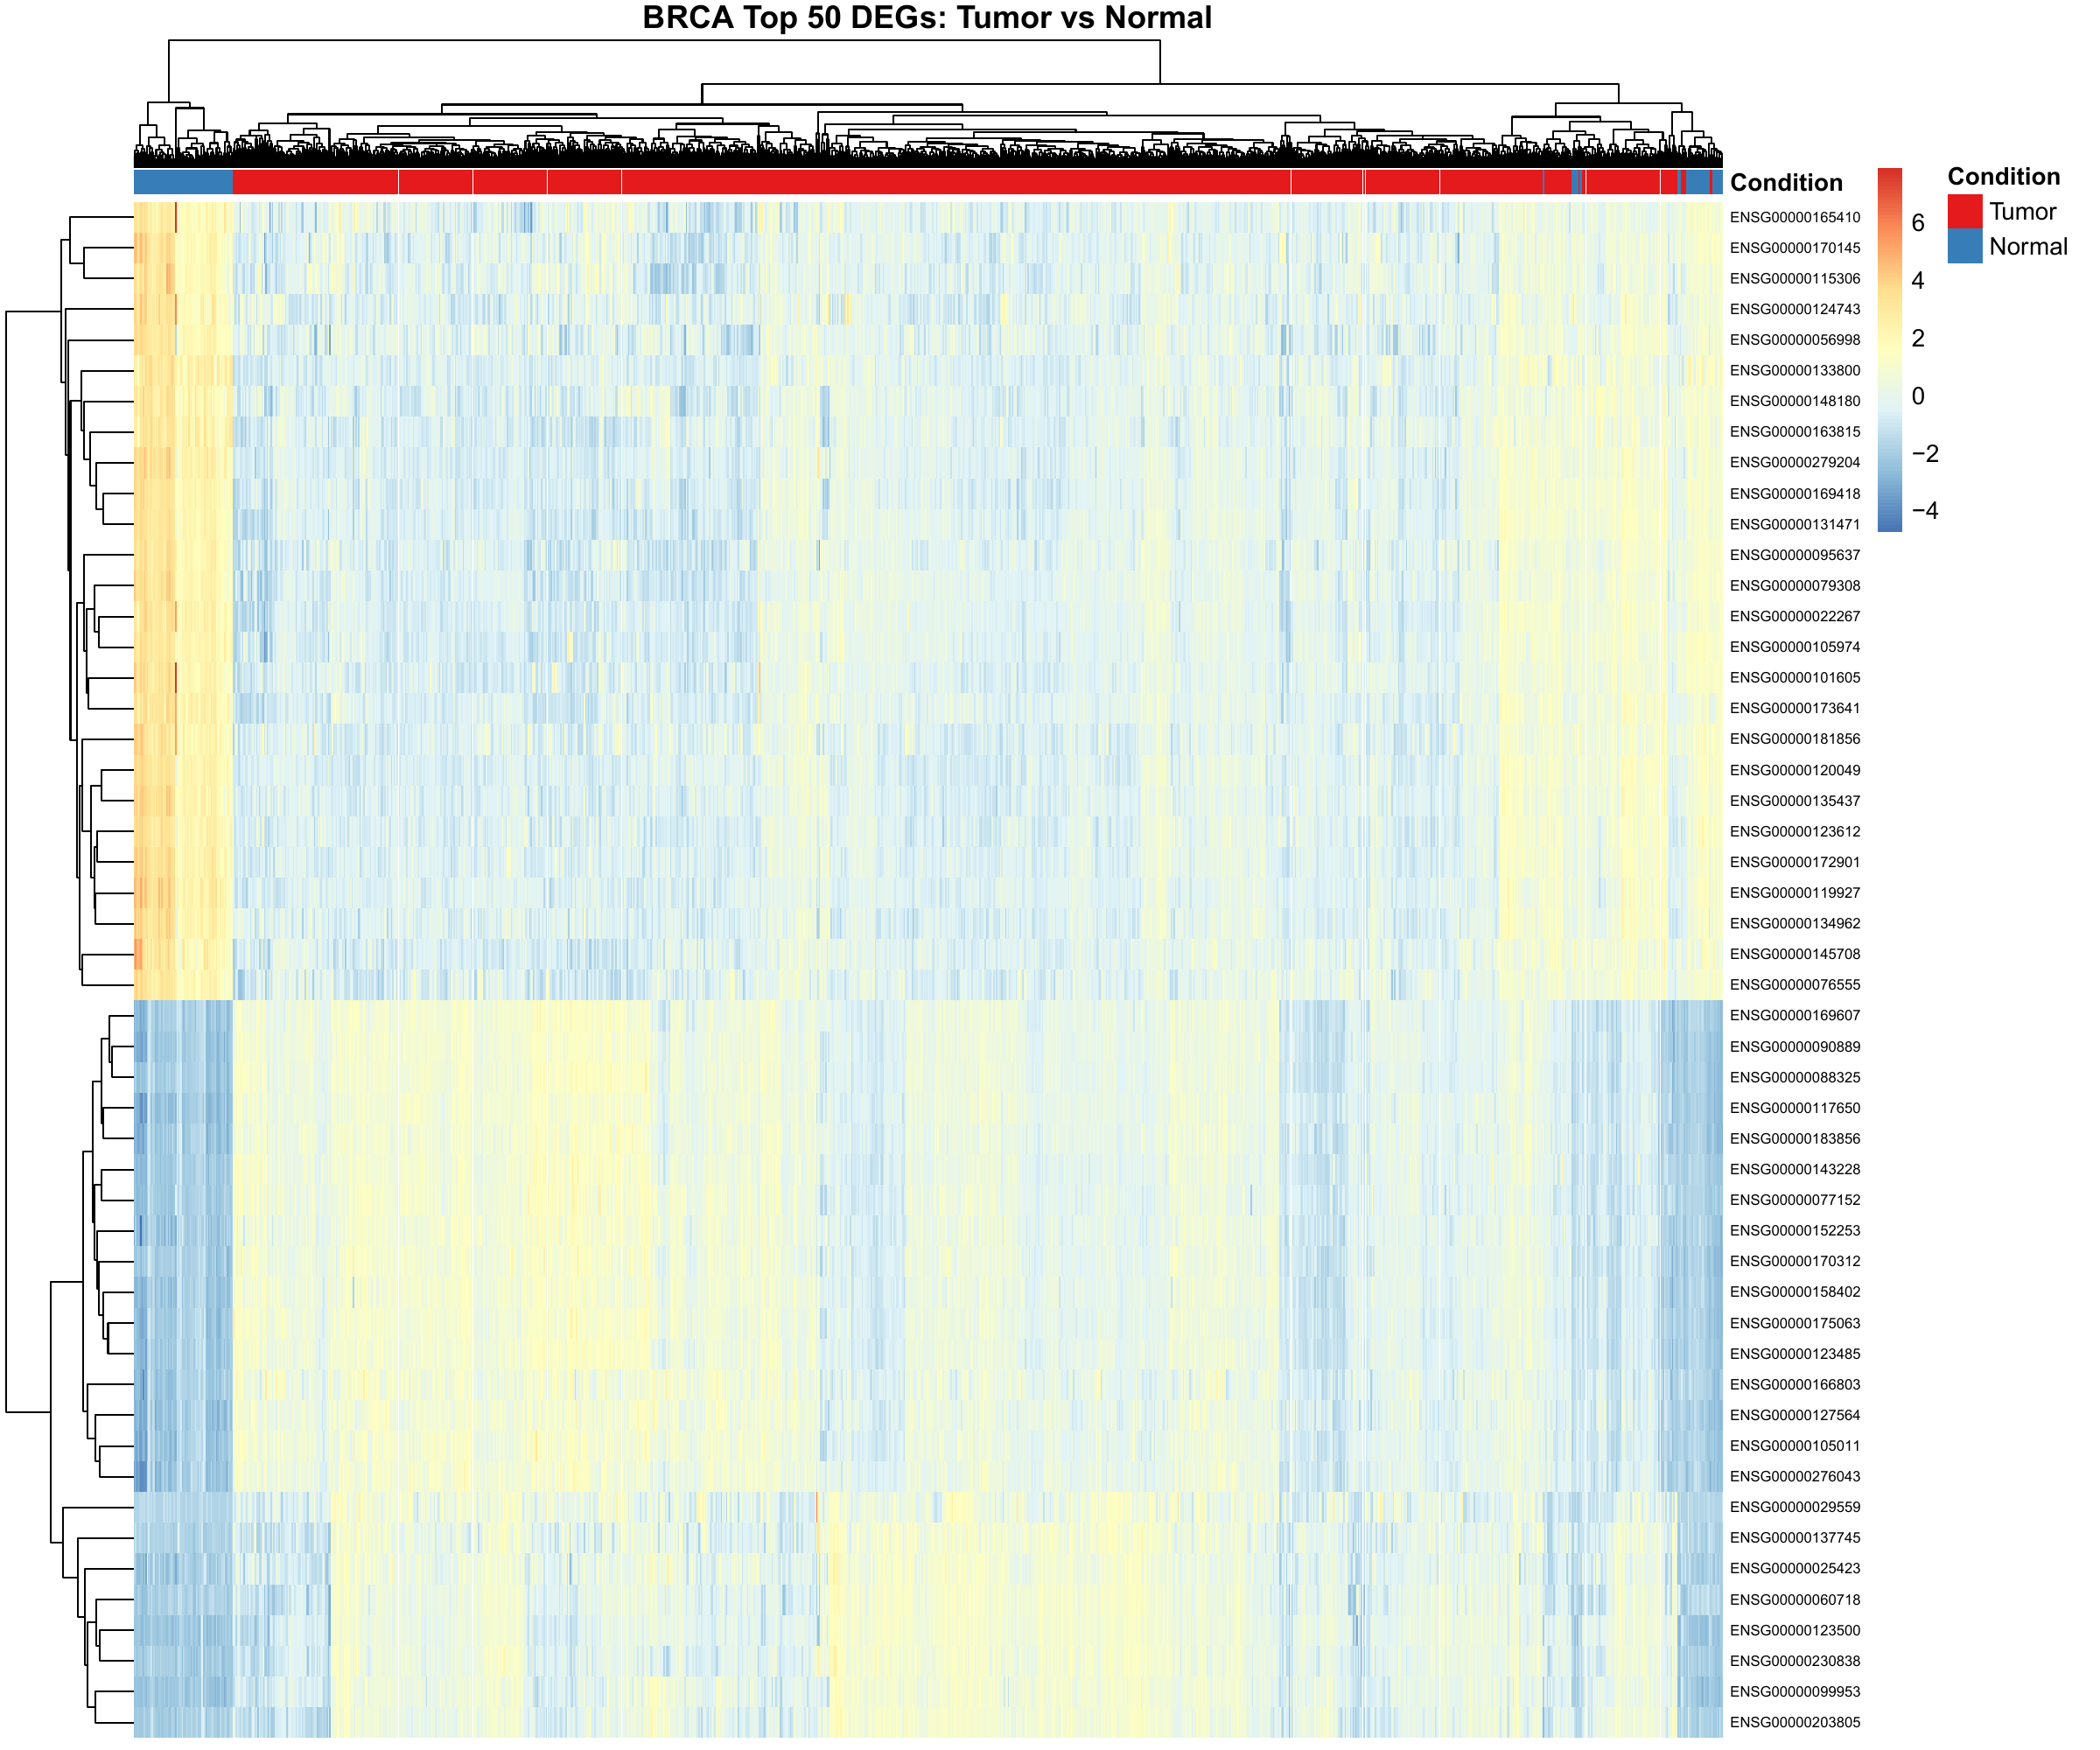
\includegraphics[width=0.75\textwidth]{figures/fig5_deg_heatmap.png}
\caption{Top 50差异表达基因热图（Z-score标准化）}
\end{figure}

功能富集分析显示上调基因显著富集于细胞周期、DNA复制等与细胞增殖相关的通路；下调基因富集于细胞外基质组织、细胞黏附等与微环境交互相关的通路。

\subsection{机器学习分类}

Random Forest和LASSO均达到75.8\%的准确率。LASSO的Kappa系数（0.332）高于Random Forest（0.281），且通过L1正则化将500个候选基因压缩至少数特征基因，验证了亚型间转录组差异的稀疏性。

\begin{figure}[H]
\centering
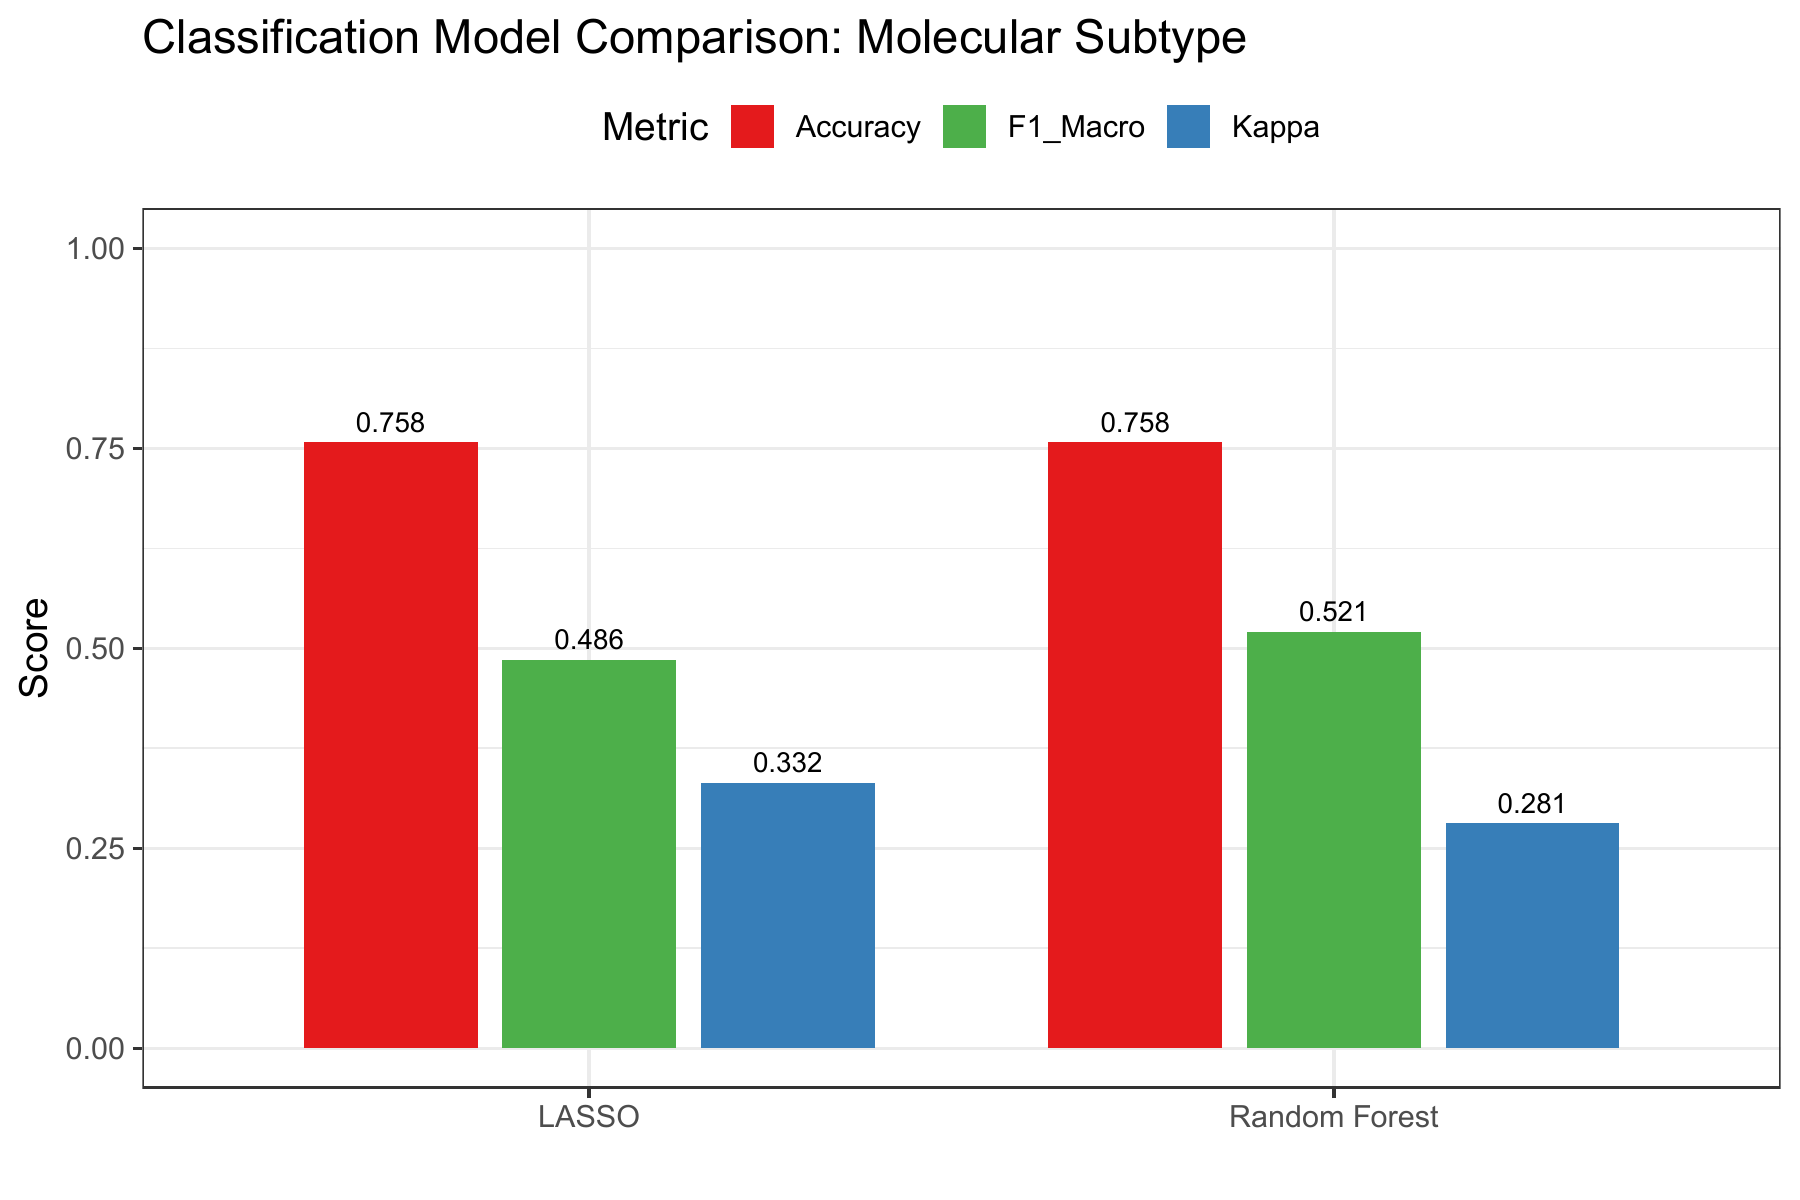
\includegraphics[width=0.75\textwidth]{figures/fig6_classification.png}
\caption{分类模型性能比较（Accuracy、Kappa、Macro F1）}
\end{figure}

\begin{figure}[H]
\centering
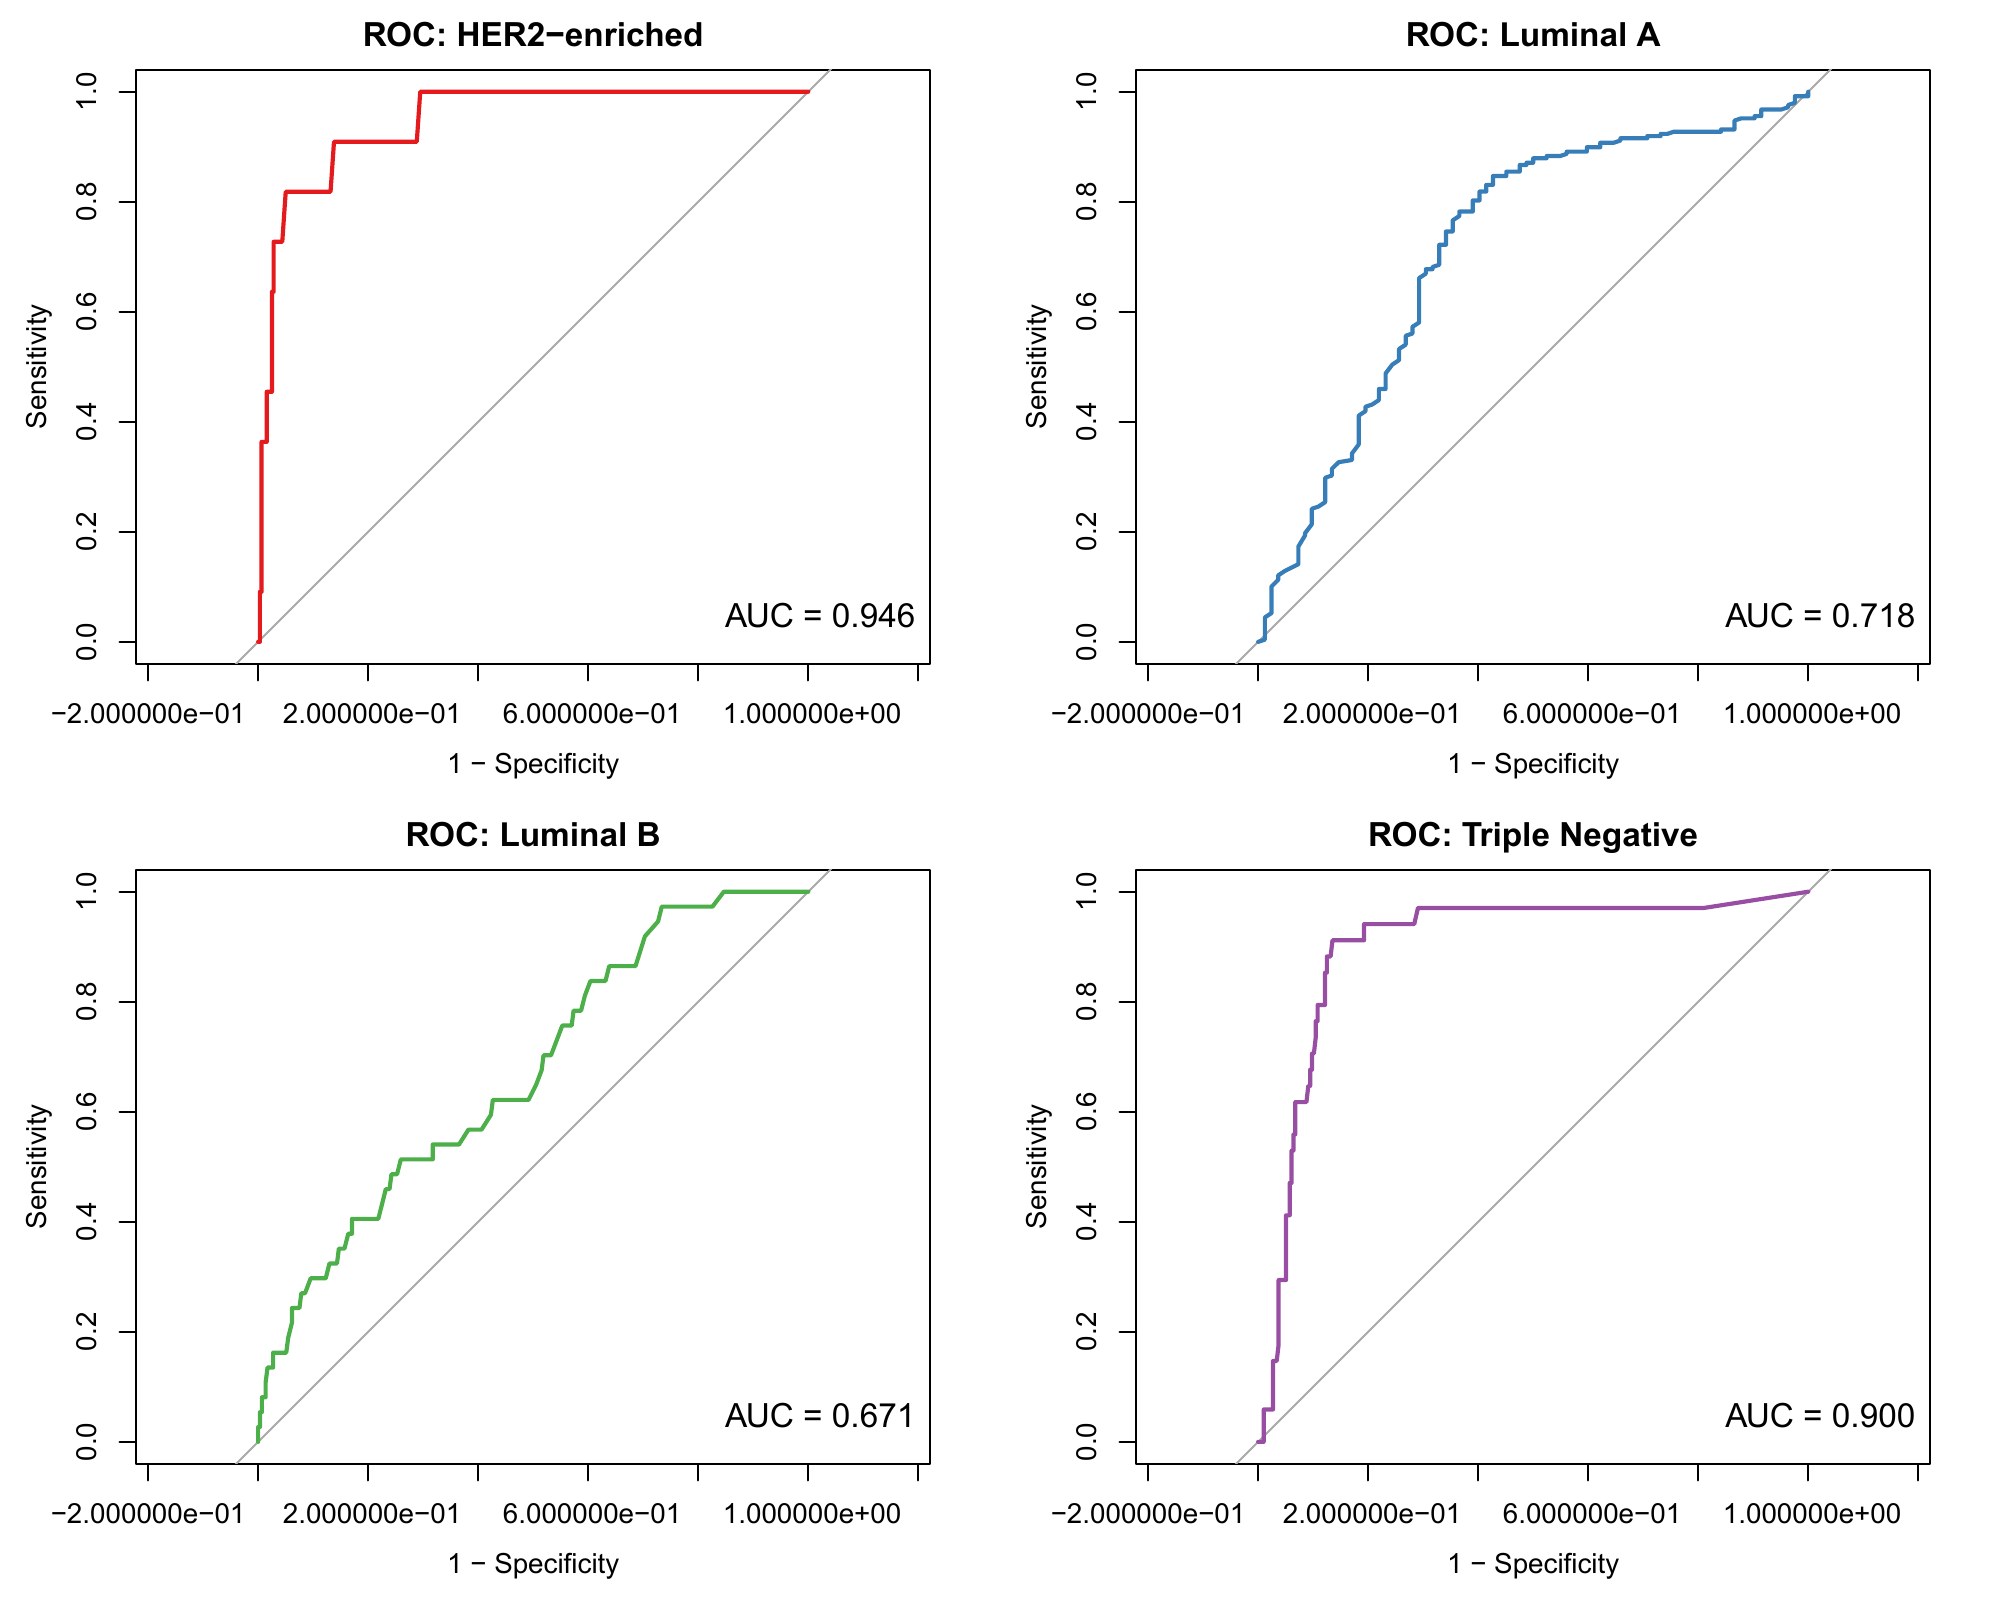
\includegraphics[width=0.7\textwidth]{figures/fig14_roc.png}
\caption{Random Forest多类别ROC曲线（One-vs-All）}
\end{figure}

\subsection{聚类分析}

PCA分析显示PC1解释15.3\%方差，PC2解释8.5\%。按分子亚型着色的散点图显示ER+与ER-亚型沿PC1方向分离明显。K-means轮廓系数在K=2时达到最大值（0.180），此后单调下降，支持ER+/ER-二分是BRCA转录组数据中最强的自然分组结构。

\begin{figure}[H]
\centering
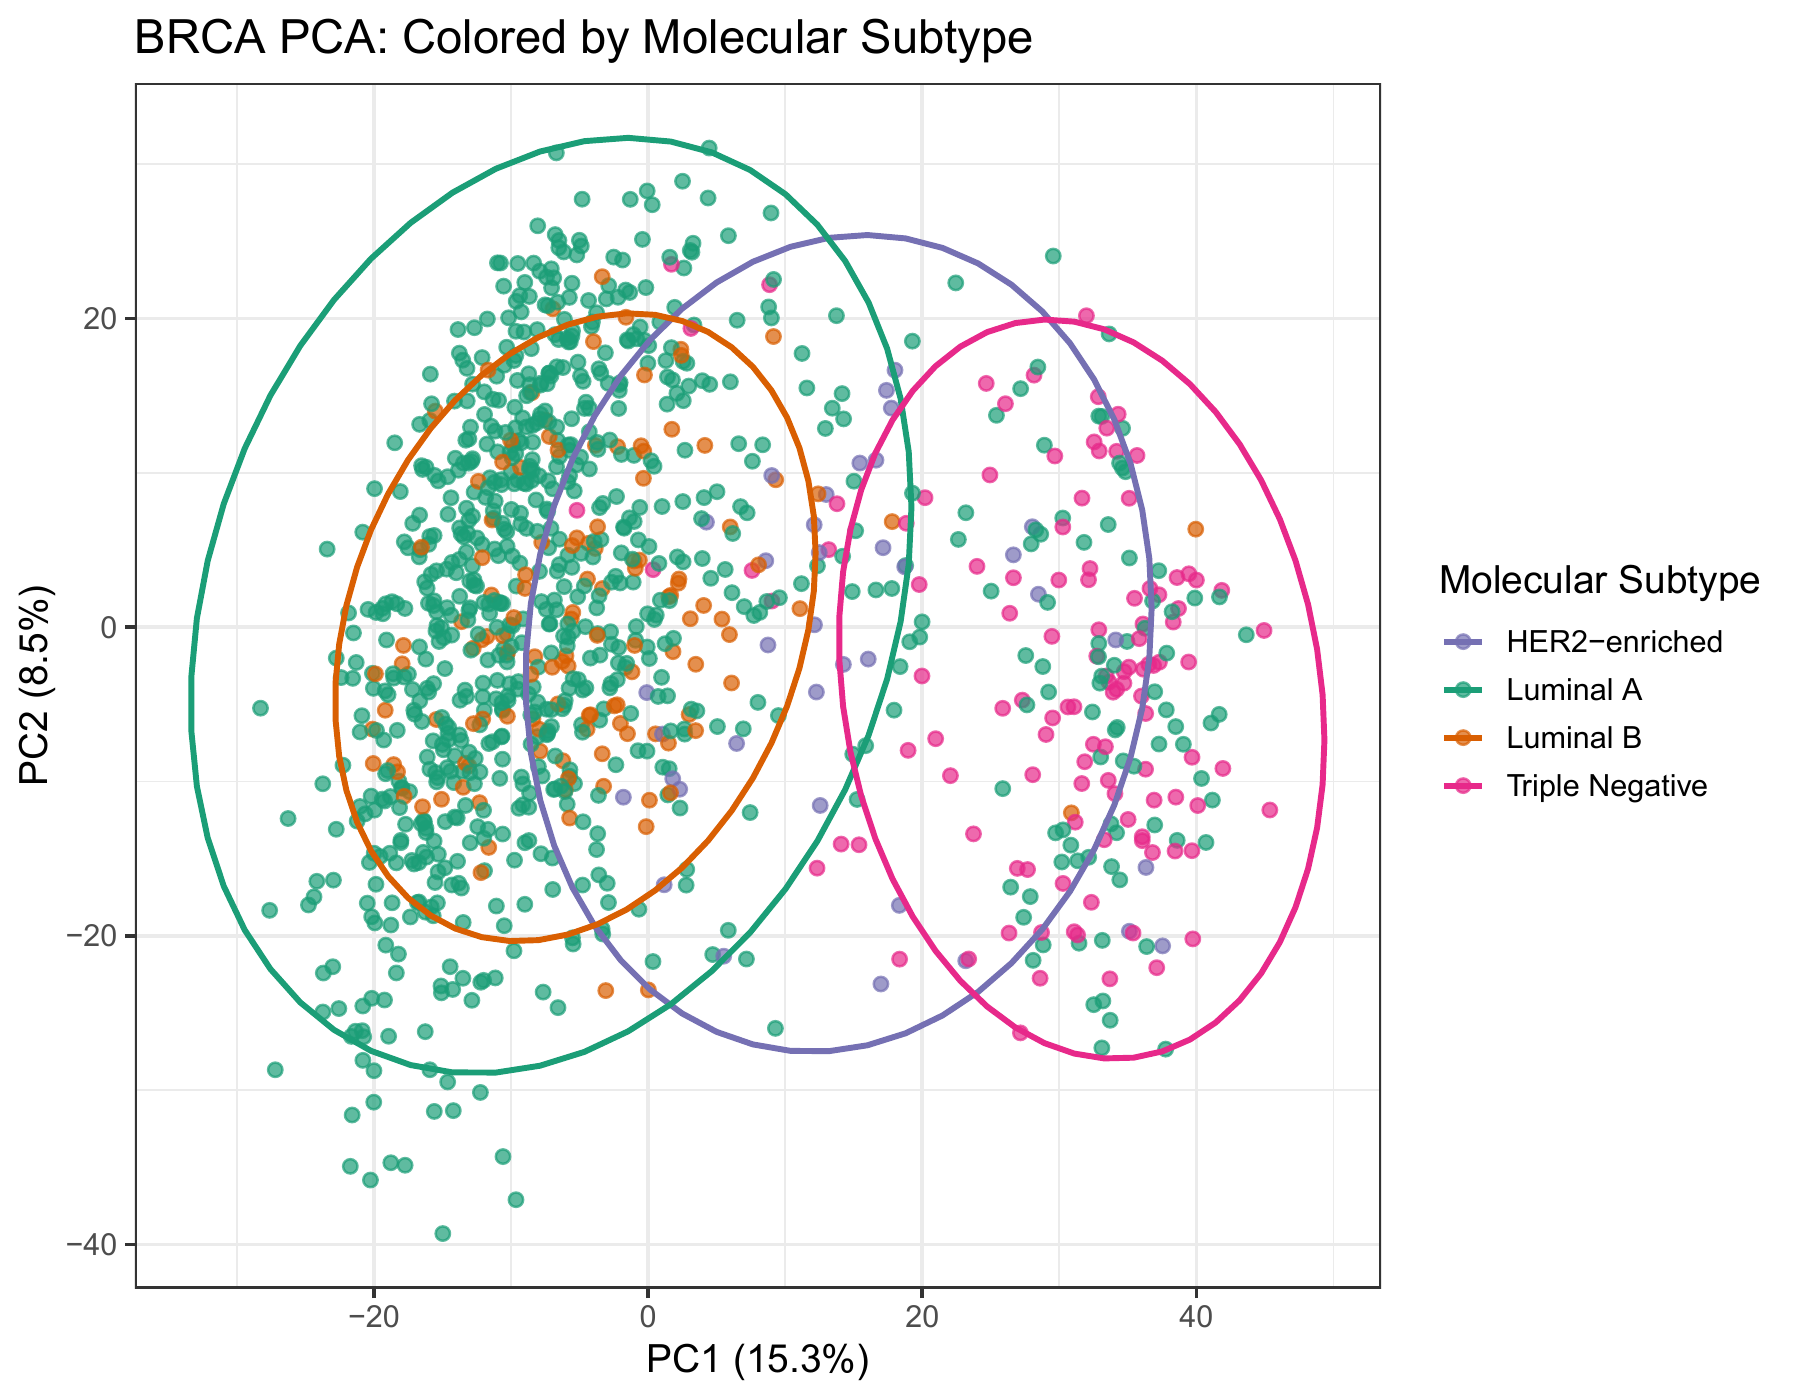
\includegraphics[width=0.8\textwidth]{figures/fig4_pca_subtype.png}
\caption{PCA散点图（按分子亚型着色），PC1=15.3\%, PC2=8.5\%}
\end{figure}

\begin{figure}[H]
\centering
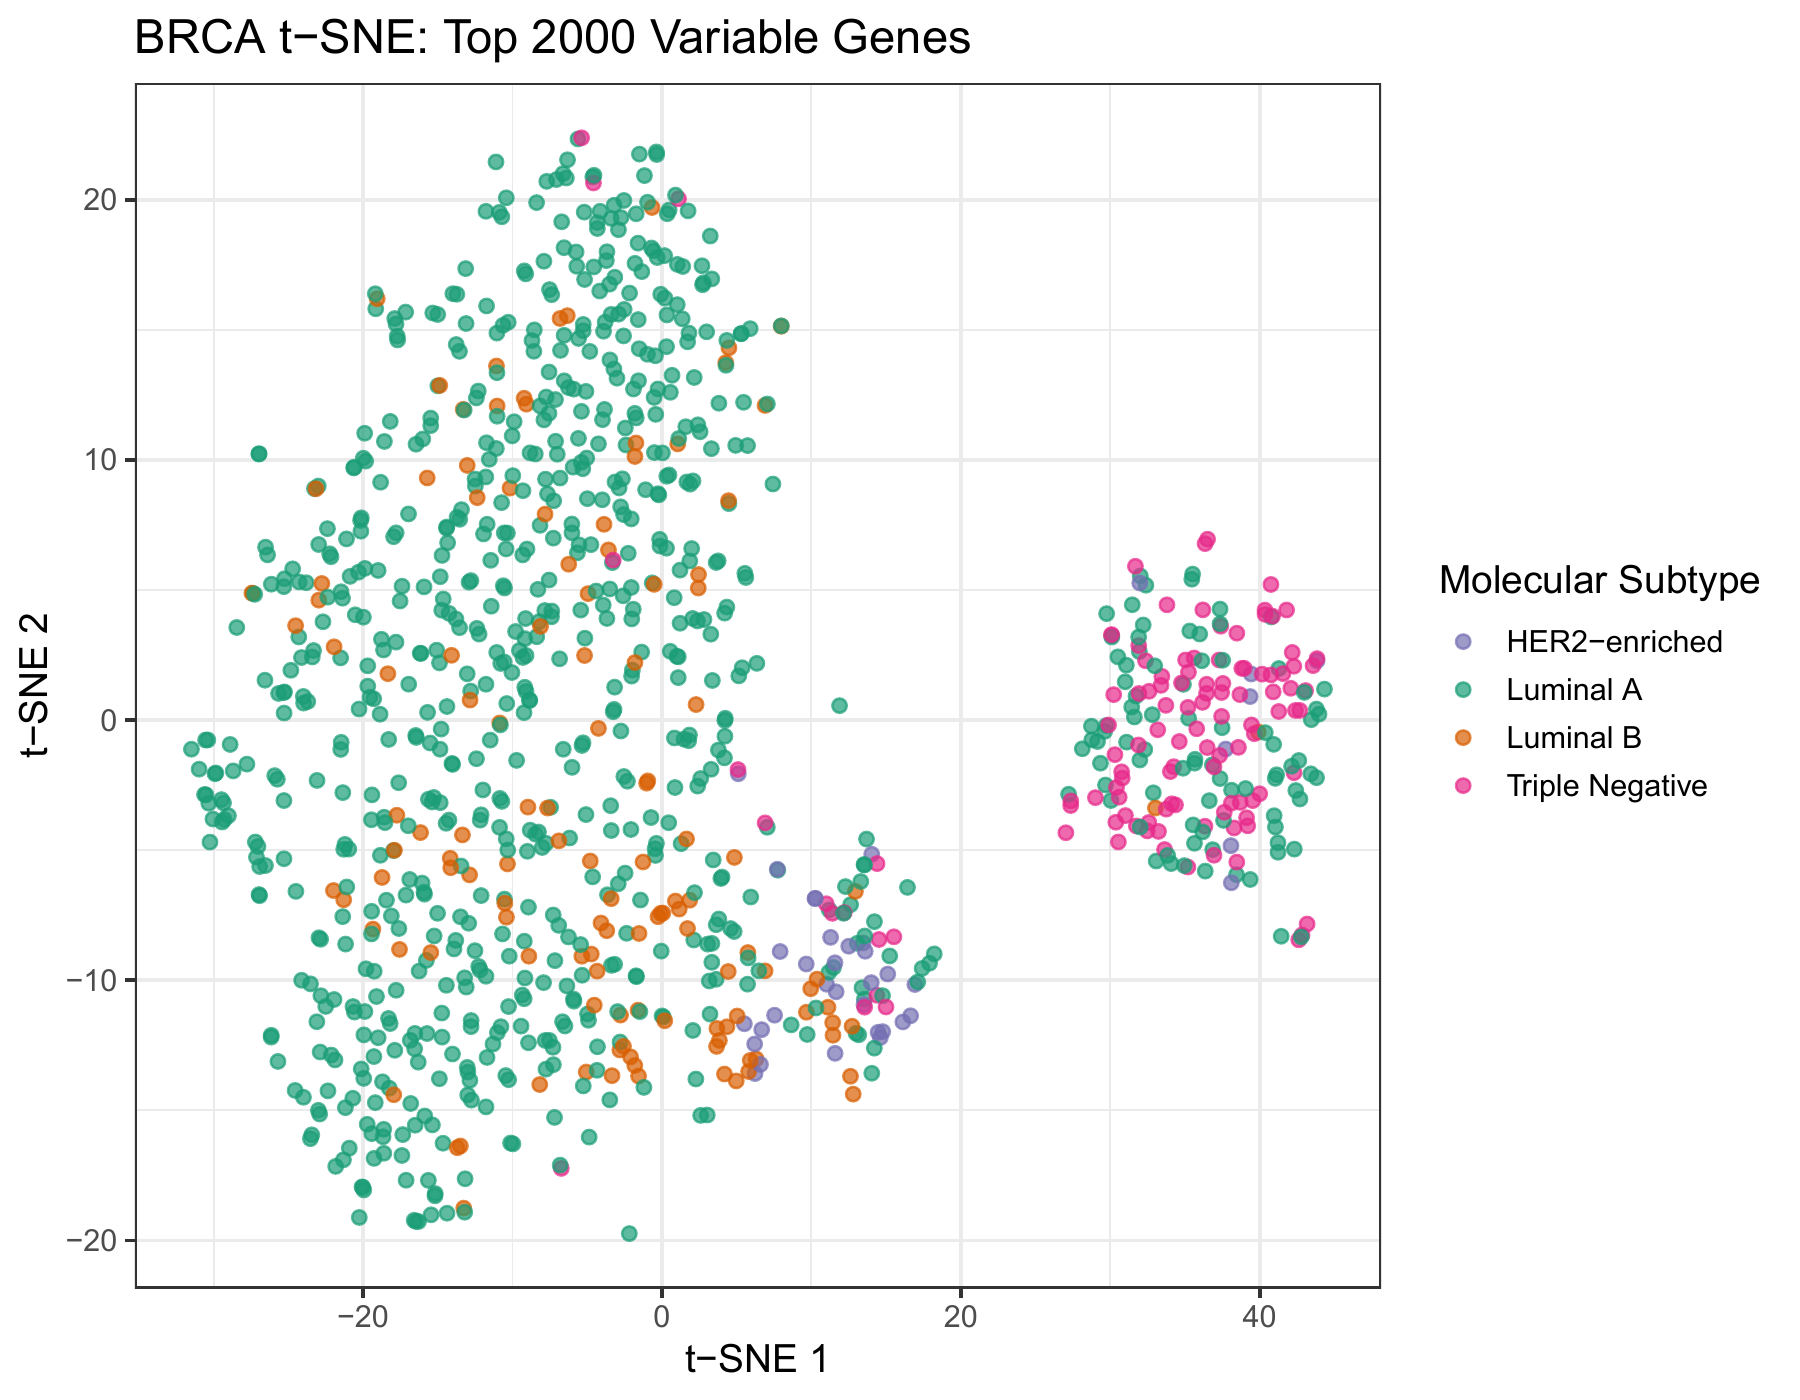
\includegraphics[width=0.8\textwidth]{figures/fig13_tsne.png}
\caption{t-SNE降维图}
\end{figure}

\begin{figure}[H]
\centering
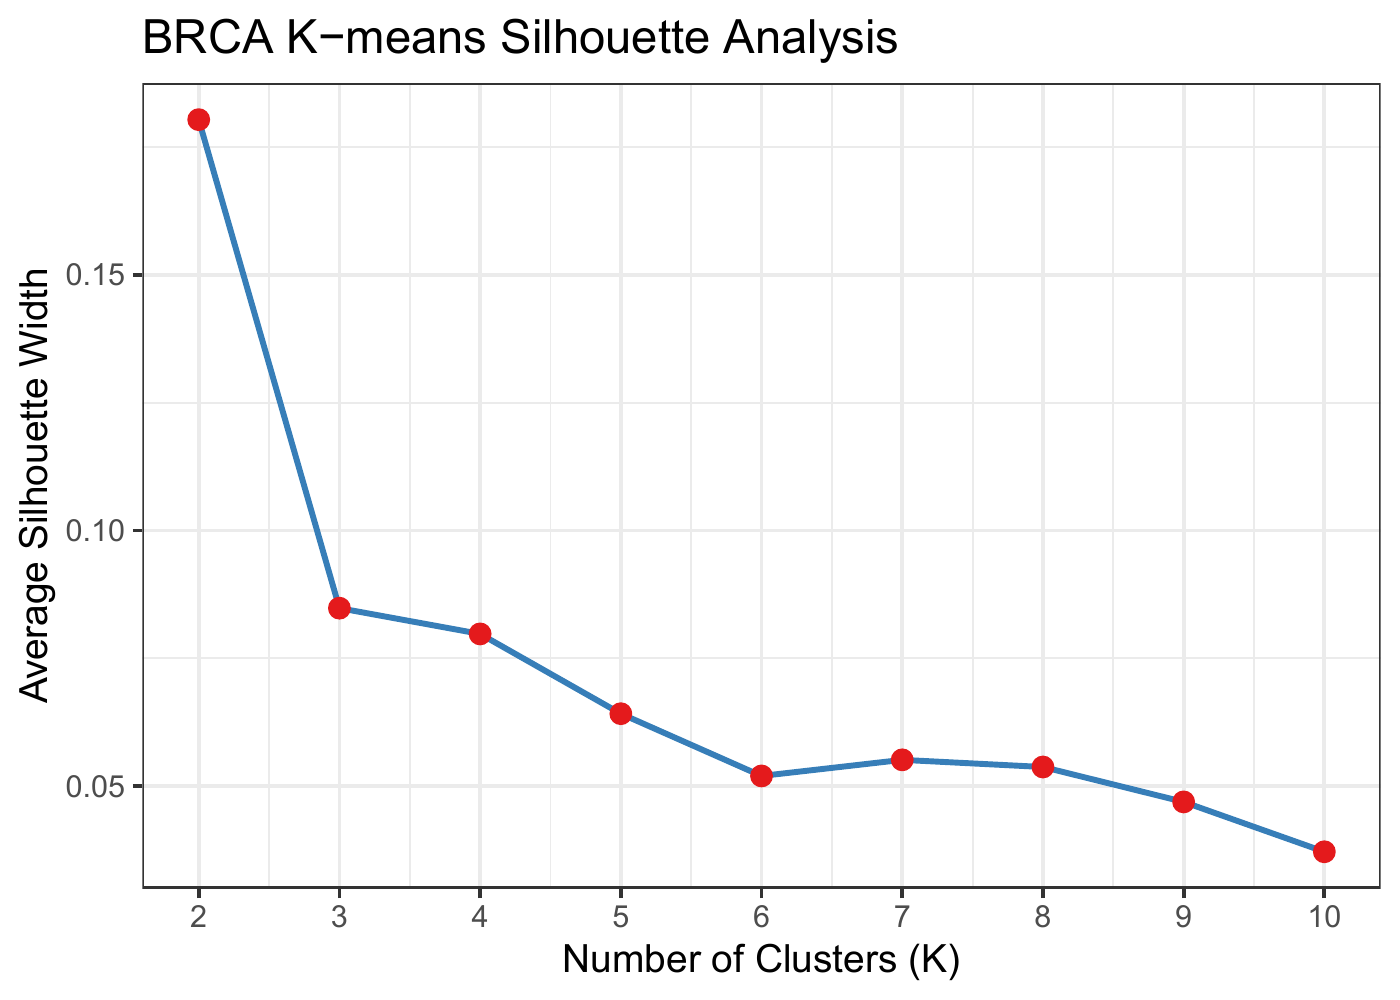
\includegraphics[width=0.7\textwidth]{figures/fig12_silhouette.png}
\caption{K-means轮廓系数分析，K=2为最优聚类数}
\end{figure}

\begin{figure}[H]
\centering
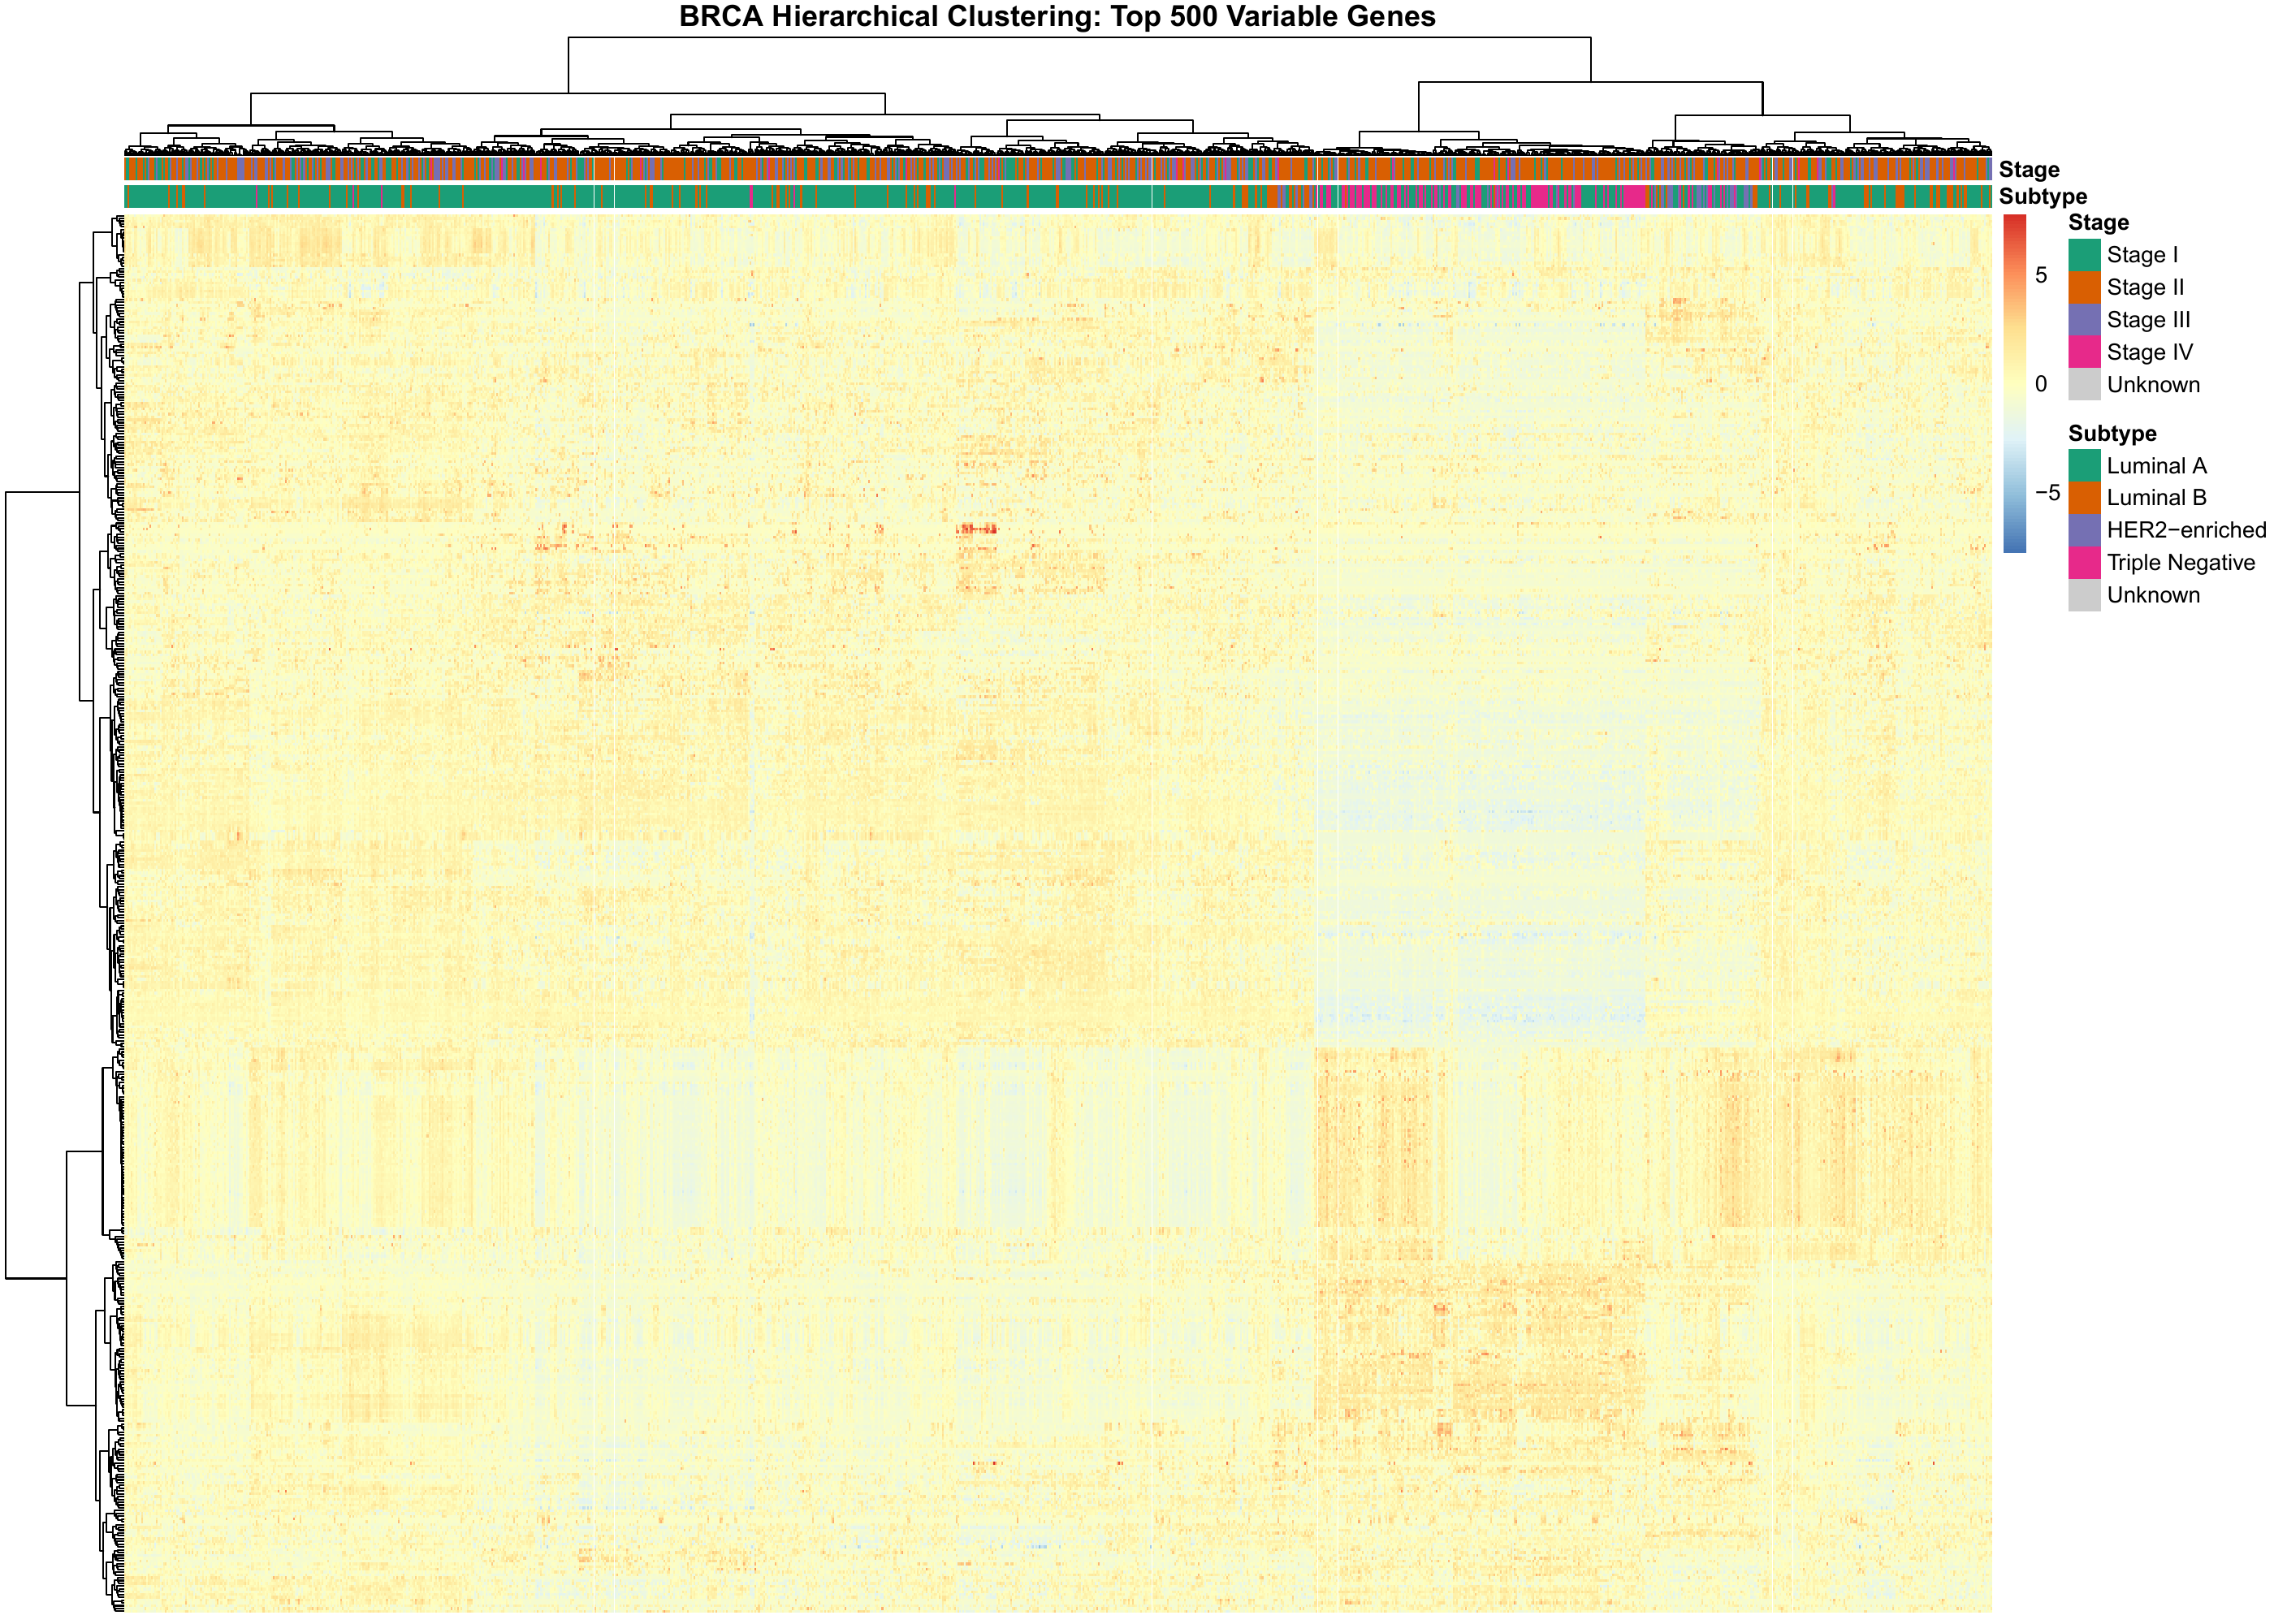
\includegraphics[width=0.9\textwidth]{figures/fig11_hclust_heatmap.png}
\caption{Top 500可变基因层次聚类热图（Ward.D2方法）}
\end{figure}

\subsection{WGCNA共表达网络分析}

软阈值选择分析确定power=8时达到scale-free $R^2=0.887$。经动态树切割和相似模块合并后，共识别9个共表达模块。模块-性状关联分析显示不同模块与分子亚型、病理分期和生存状态之间存在显著相关性。

\begin{figure}[H]
\centering
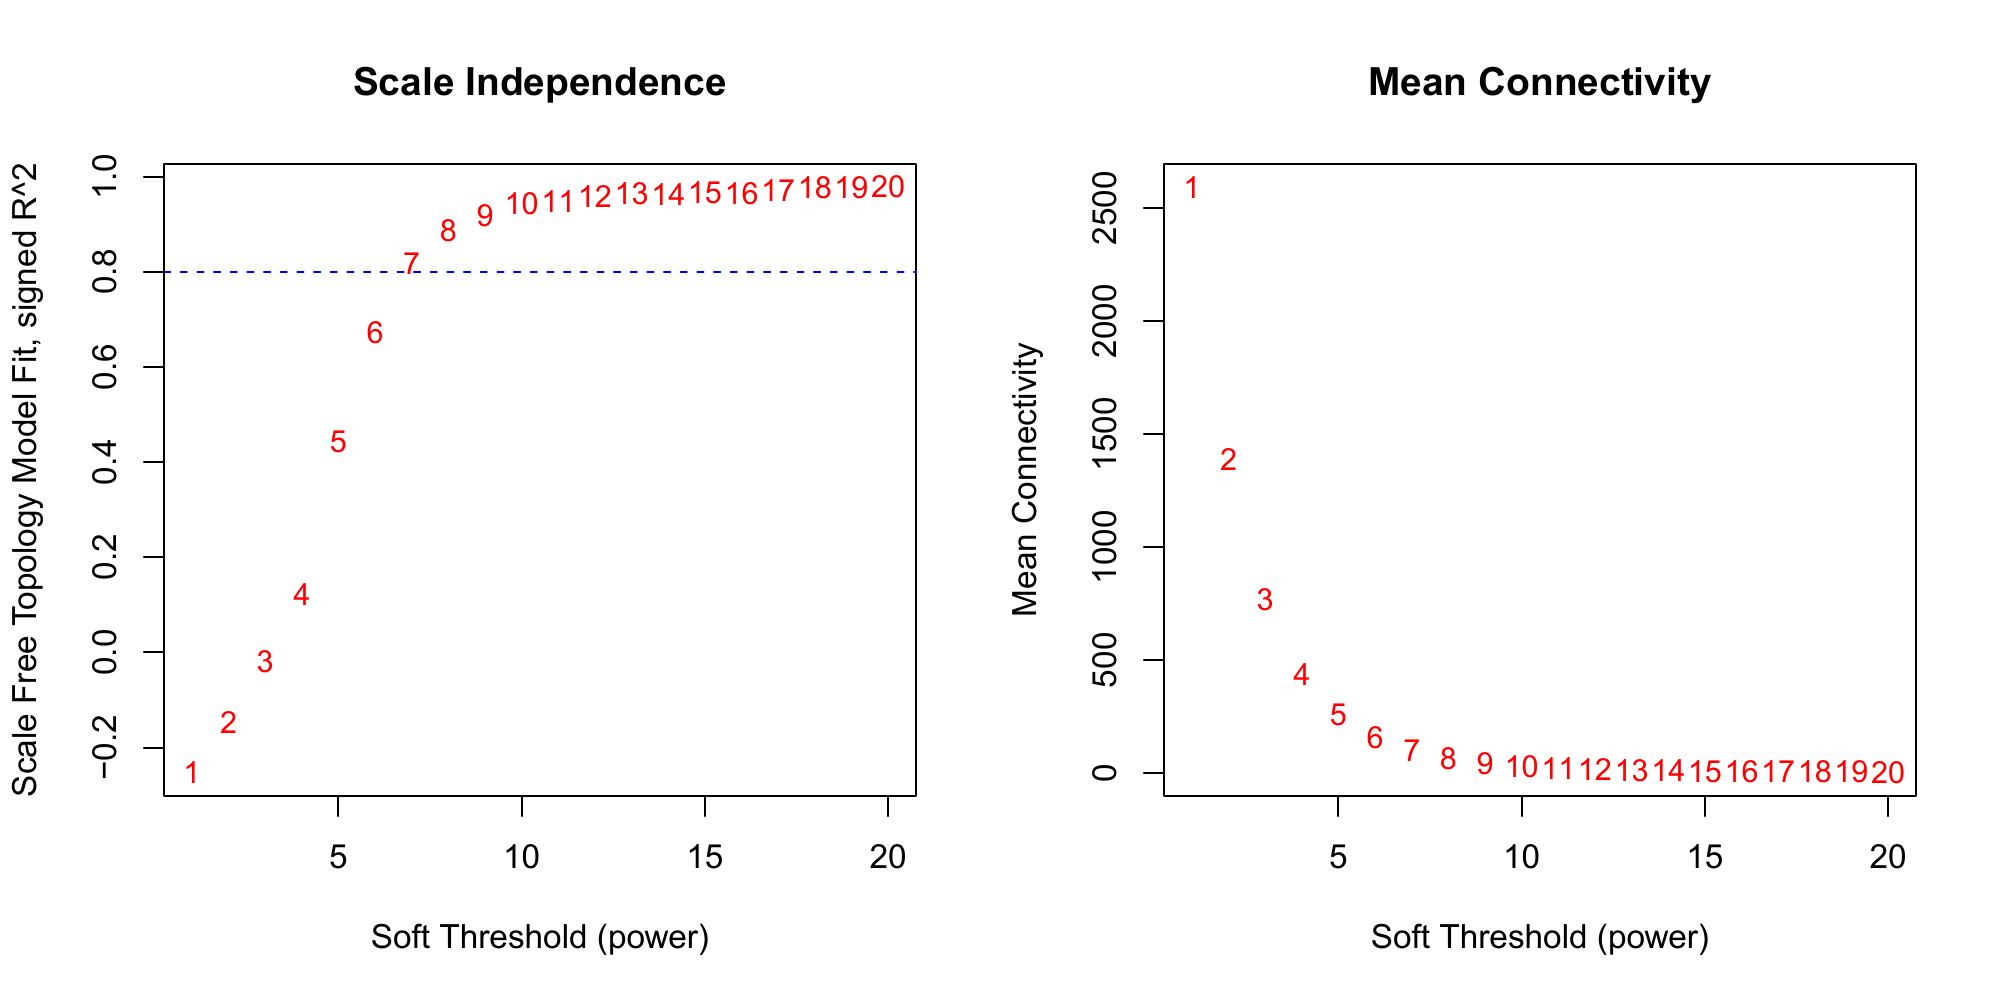
\includegraphics[width=0.8\textwidth]{figures/fig8_wgcna_soft_power.png}
\caption{WGCNA软阈值选择，power=8}
\end{figure}

\begin{figure}[H]
\centering
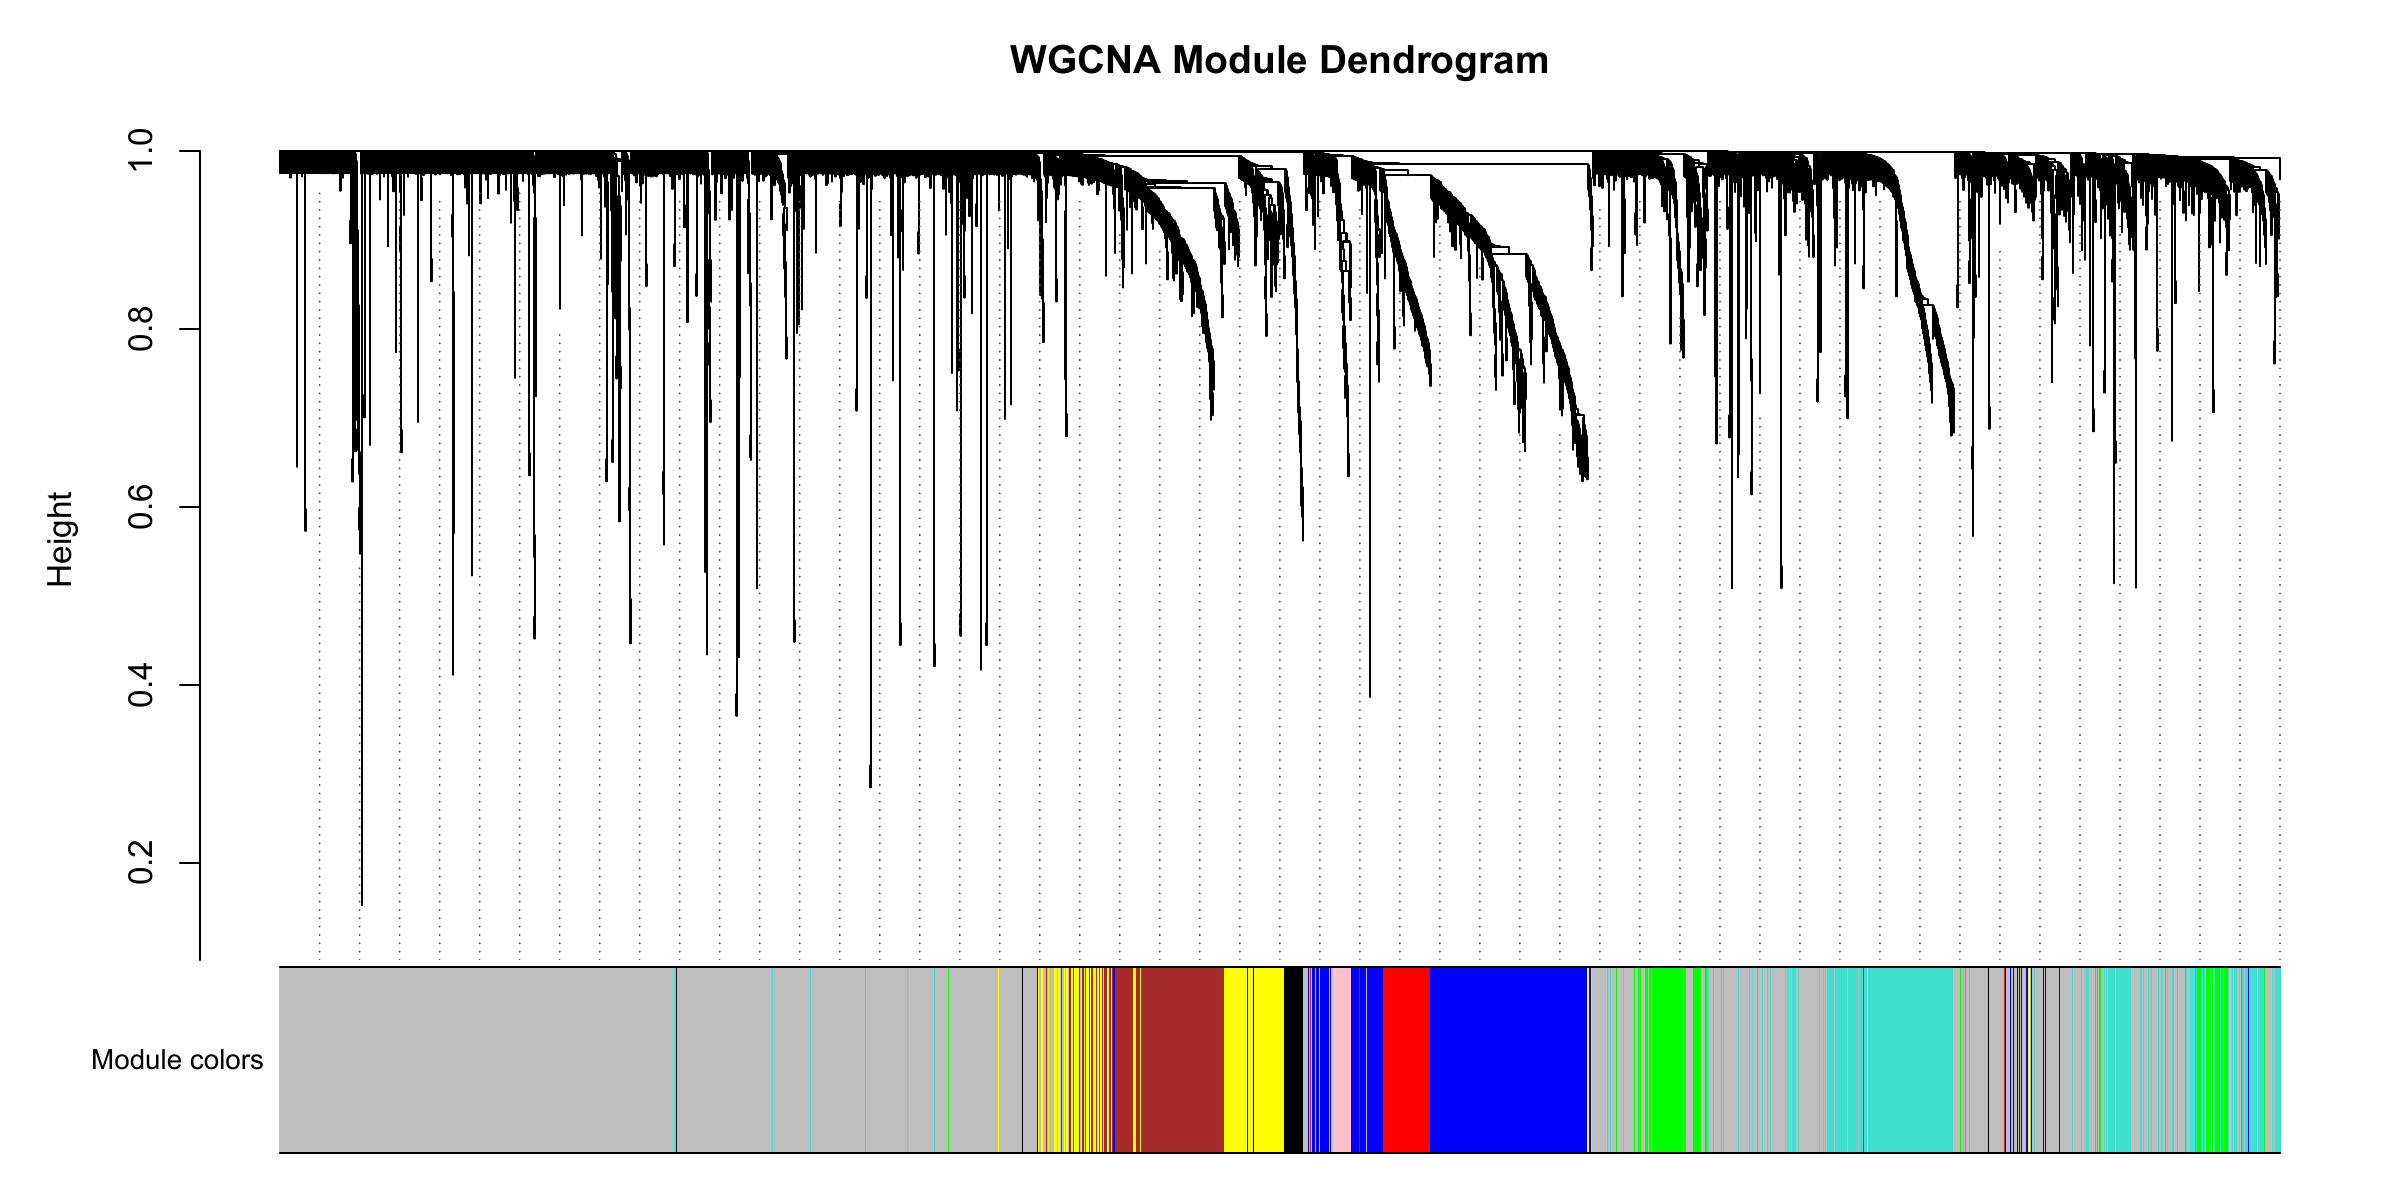
\includegraphics[width=0.85\textwidth]{figures/fig16_wgcna_dendrogram.png}
\caption{WGCNA模块树状图与颜色标识（共9个模块）}
\end{figure}

\begin{figure}[H]
\centering
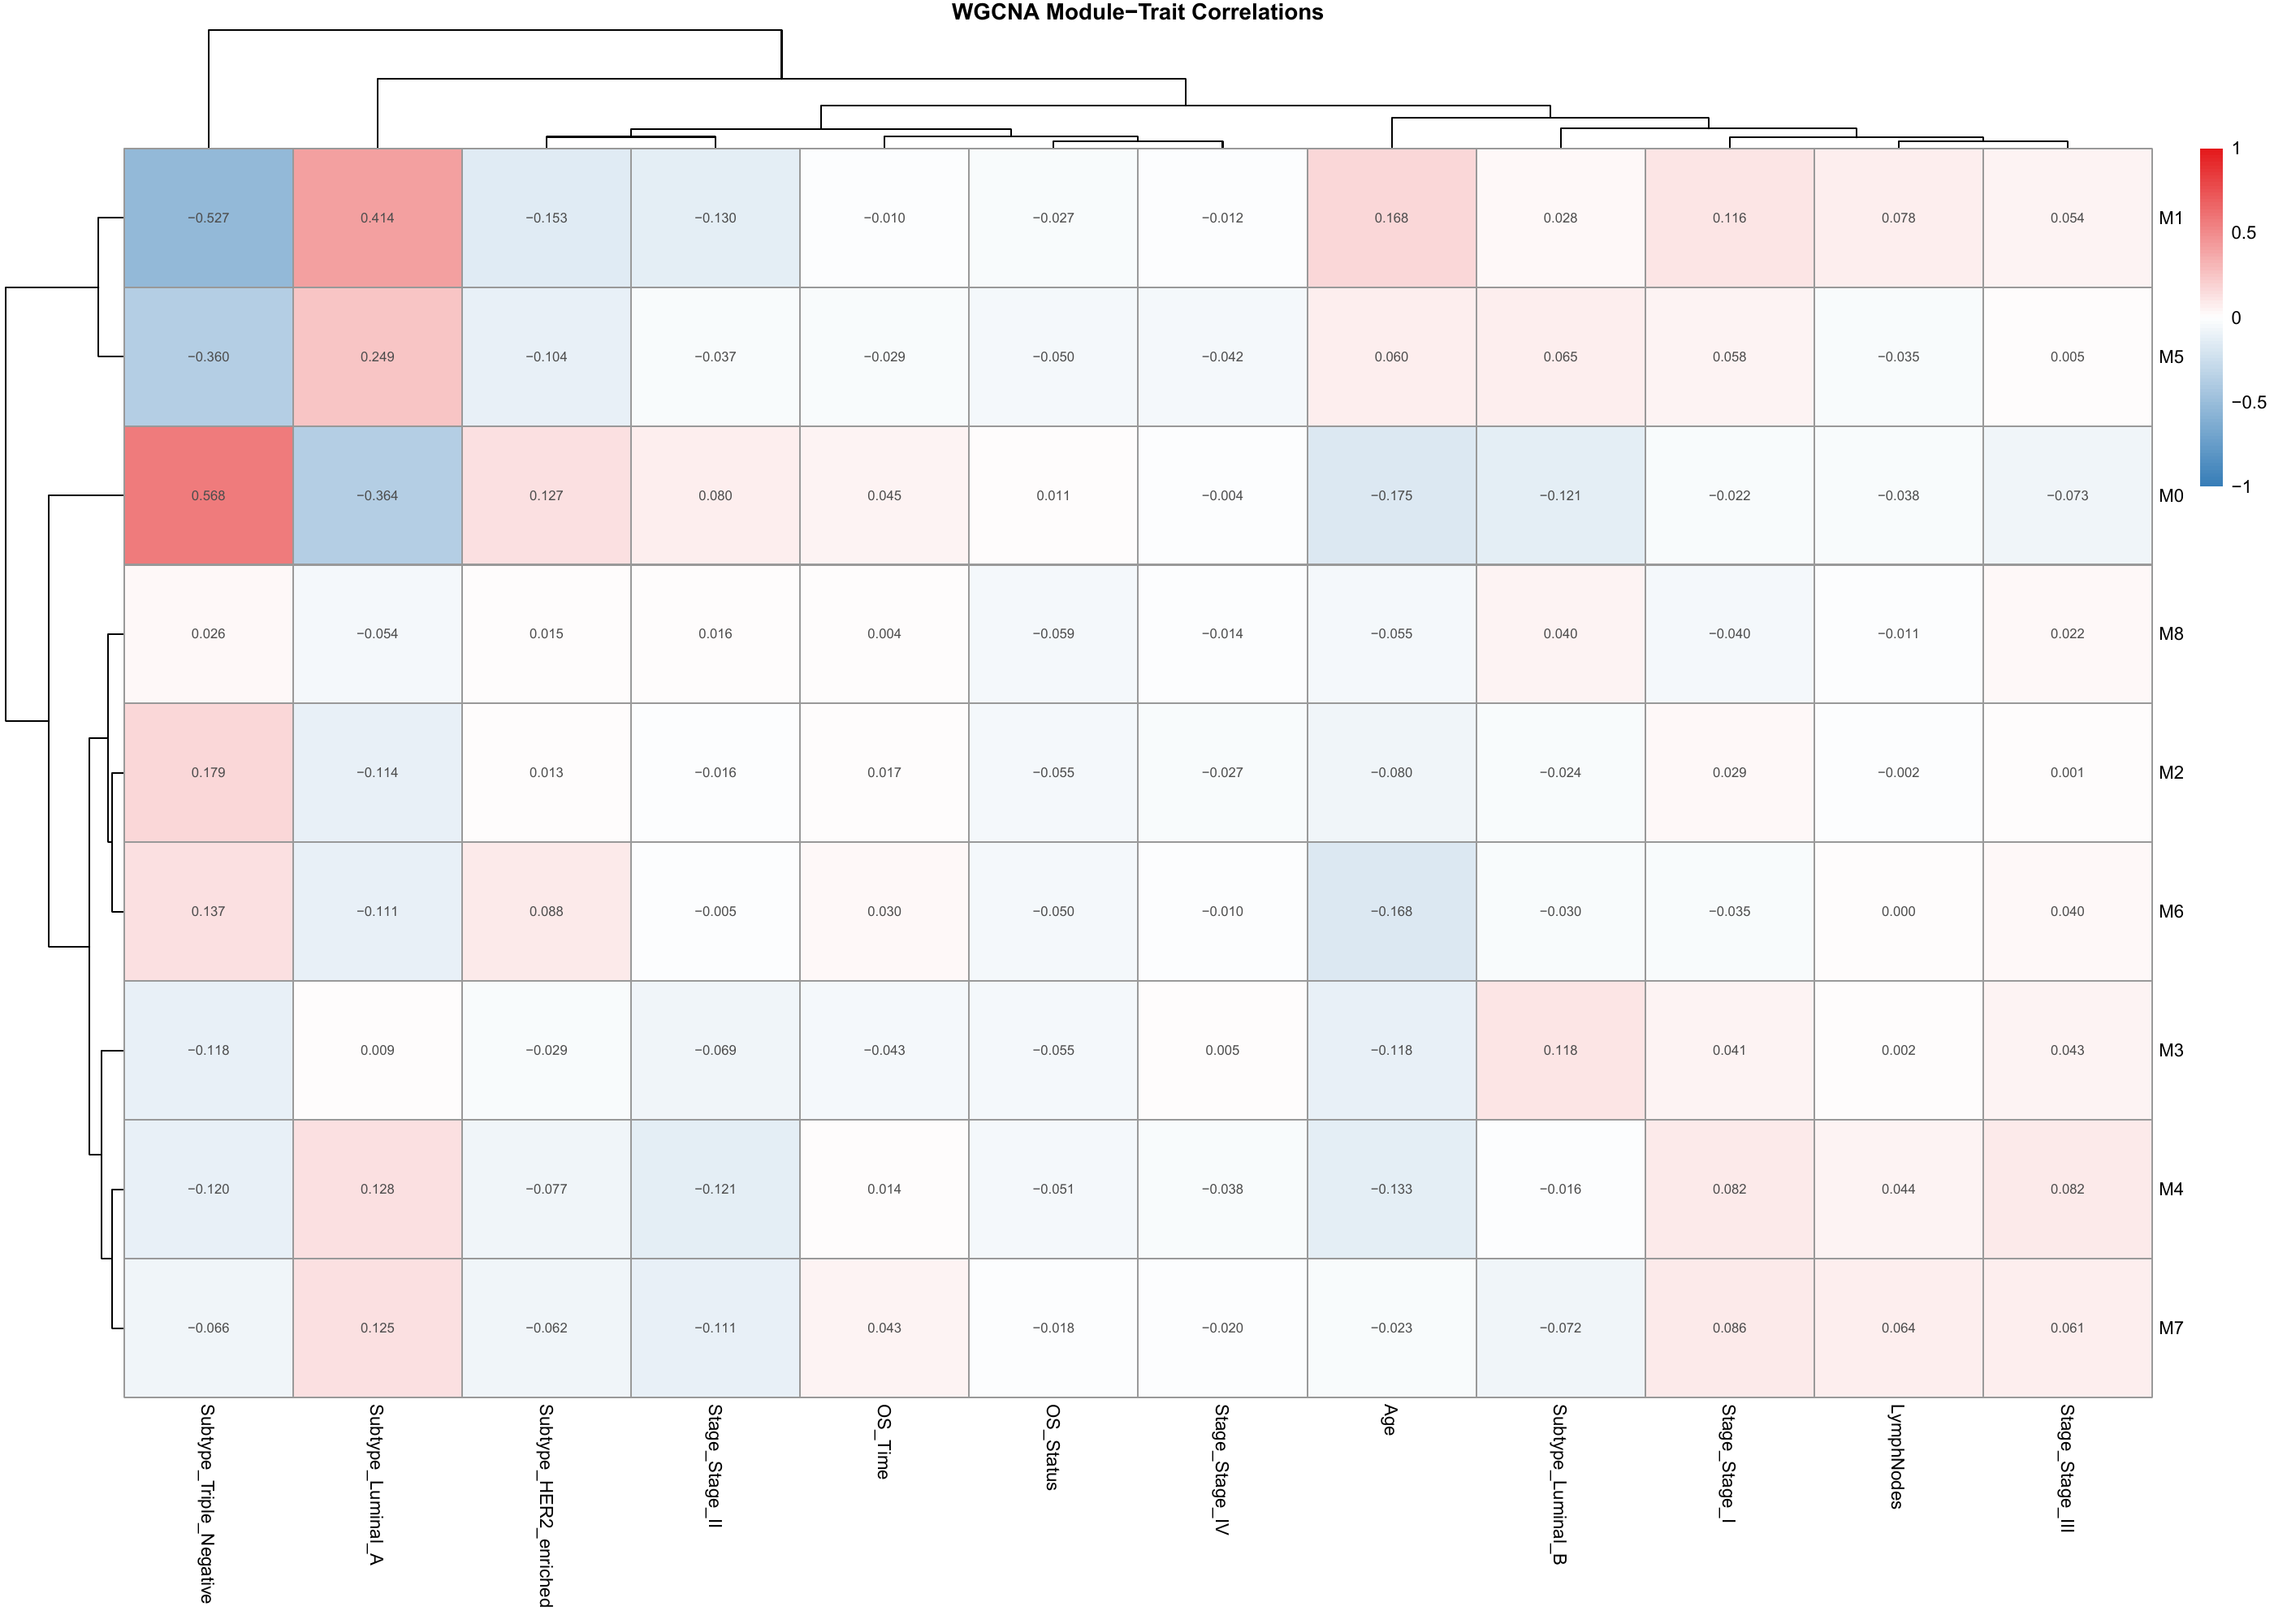
\includegraphics[width=0.85\textwidth]{figures/fig7_wgcna_module_trait.png}
\caption{WGCNA模块-性状相关性热图}
\end{figure}

在关键模块中识别了枢纽基因：Module M2（blue, 553个基因）枢纽基因（ENSG00000167208）的模块隶属度达0.959；Module M8（pink, 44个基因）枢纽基因MM=0.966；Module M3（brown, 336个基因）枢纽基因MM=0.940。

\begin{figure}[H]
\centering
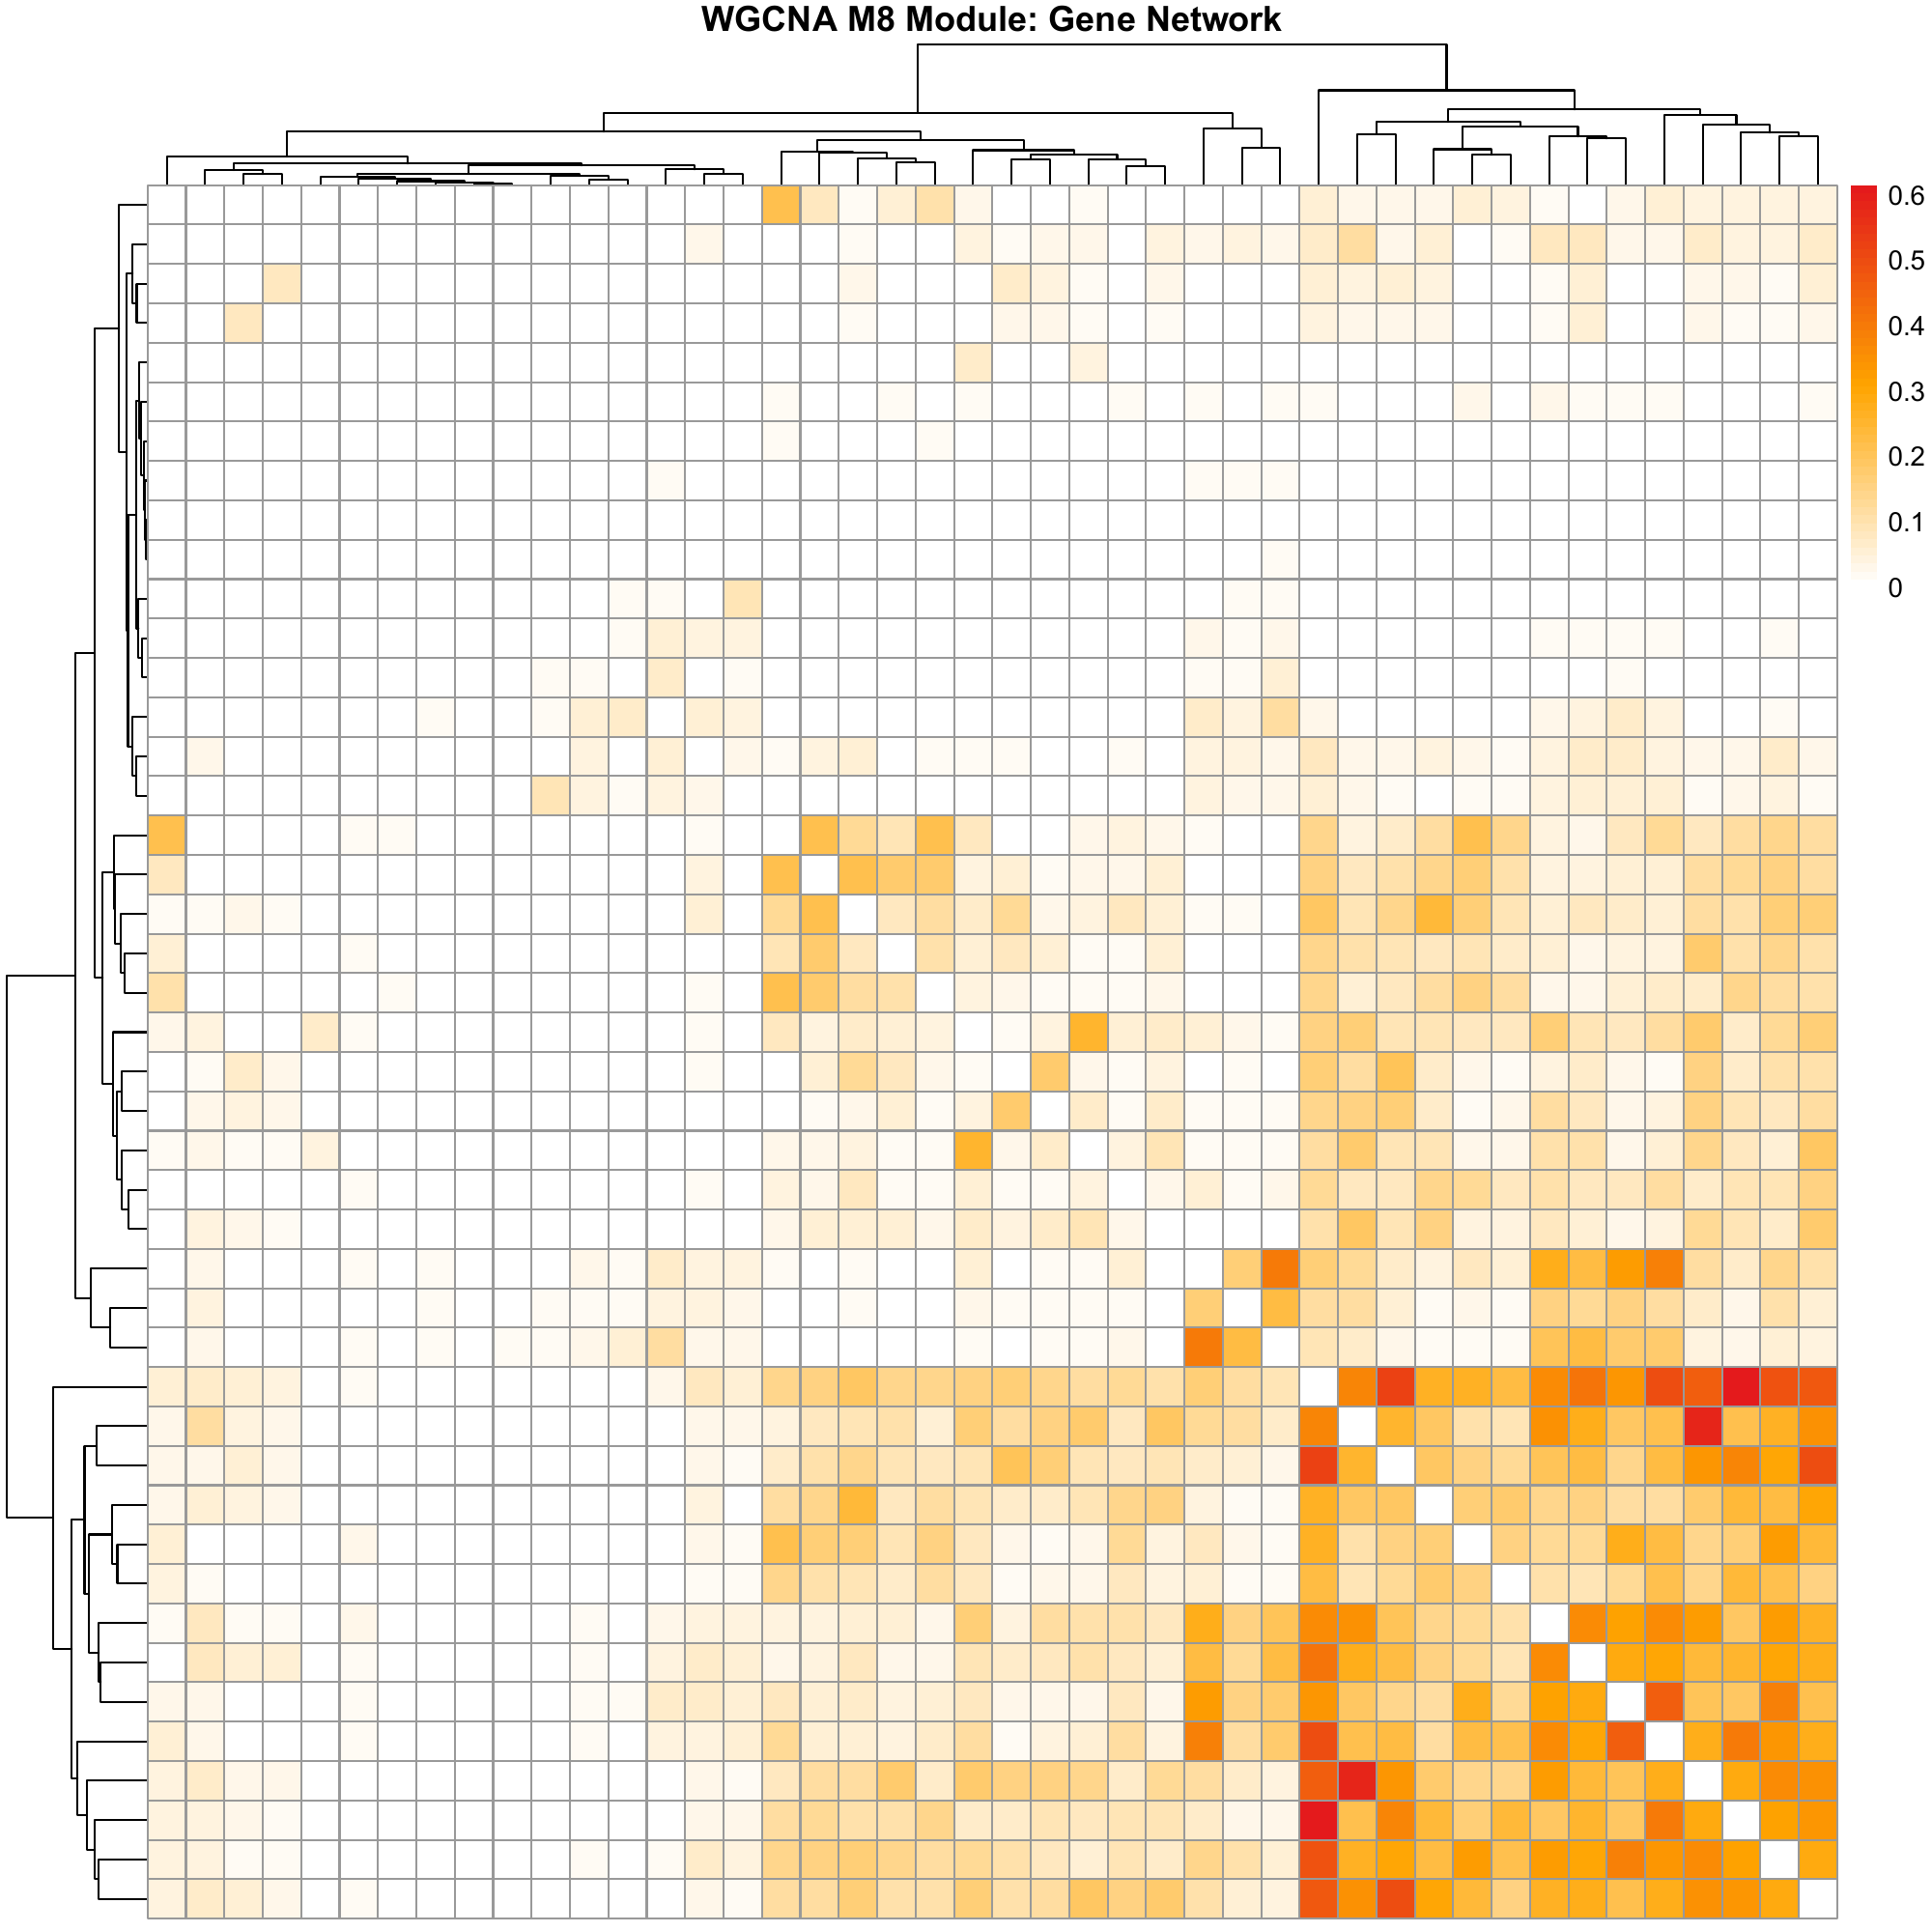
\includegraphics[width=0.7\textwidth]{figures/fig17_wgcna_network.png}
\caption{关键模块基因共表达网络热图（Top 50枢纽基因）}
\end{figure}

\subsection{生存分析}

Kaplan-Meier分析显示病理分期与总生存之间存在显著关联（log-rank p$<0.001$），Stage IV预后最差。

\begin{figure}[H]
\centering

\includegraphics[width=0.85\textwidth]{figures/km_curves_stage.png}
\caption{Kaplan-Meier生存曲线（按病理分期分组）}
\end{figure}

\begin{figure}[H]
\centering
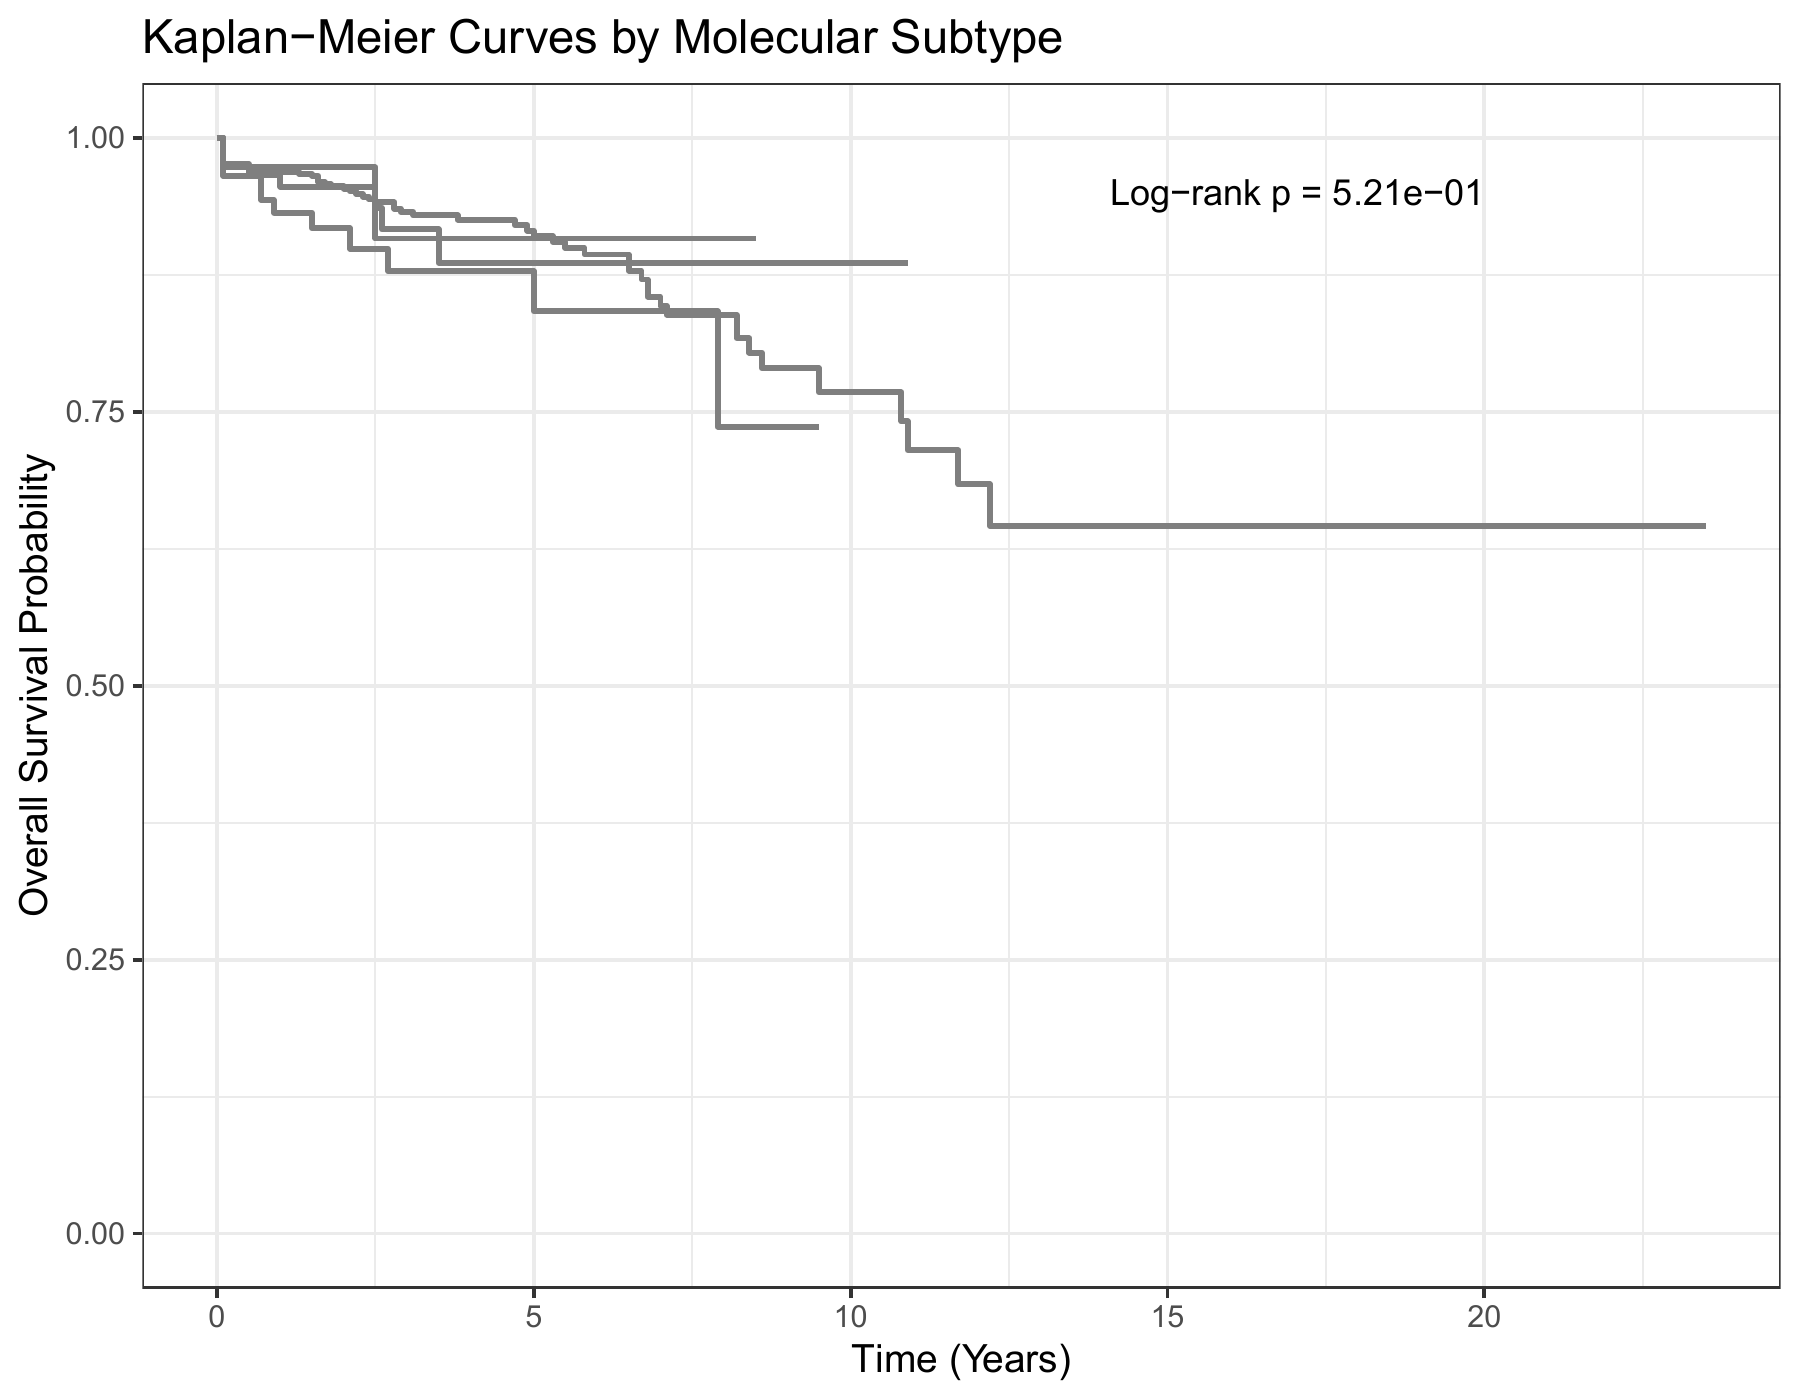
\includegraphics[width=0.85\textwidth]{figures/km_curves_subtype.png}
\caption{Kaplan-Meier生存曲线（按分子亚型分组）}
\end{figure}

多变量Cox回归（C-index=0.767, 似然比p$=3.61\times10^{-12}$）结果如表2和图17所示。Stage IV风险比达29.82（95\%CI: 10.14--87.76, p$=7.02\times10^{-10}$）。

\begin{table}[H]
\centering
\caption{多变量Cox回归结果}
\begin{tabular}{lcccc}
\toprule
变量 & HR & 95\% CI下限 & 95\% CI上限 & p值 \\
\midrule
年龄 & 1.04 & 1.02 & 1.06 & $7.4\times10^{-6}$ \\
Stage II & 3.24 & 1.28 & 8.19 & 0.013 \\
Stage III & 6.00 & 2.31 & 15.58 & $2.4\times10^{-4}$ \\
Stage IV & 29.82 & 10.14 & 87.76 & $7.0\times10^{-10}$ \\
Triple Negative & 2.00 & 1.08 & 3.71 & 0.028 \\
\bottomrule
\end{tabular}
\end{table}

\begin{figure}[H]
\centering
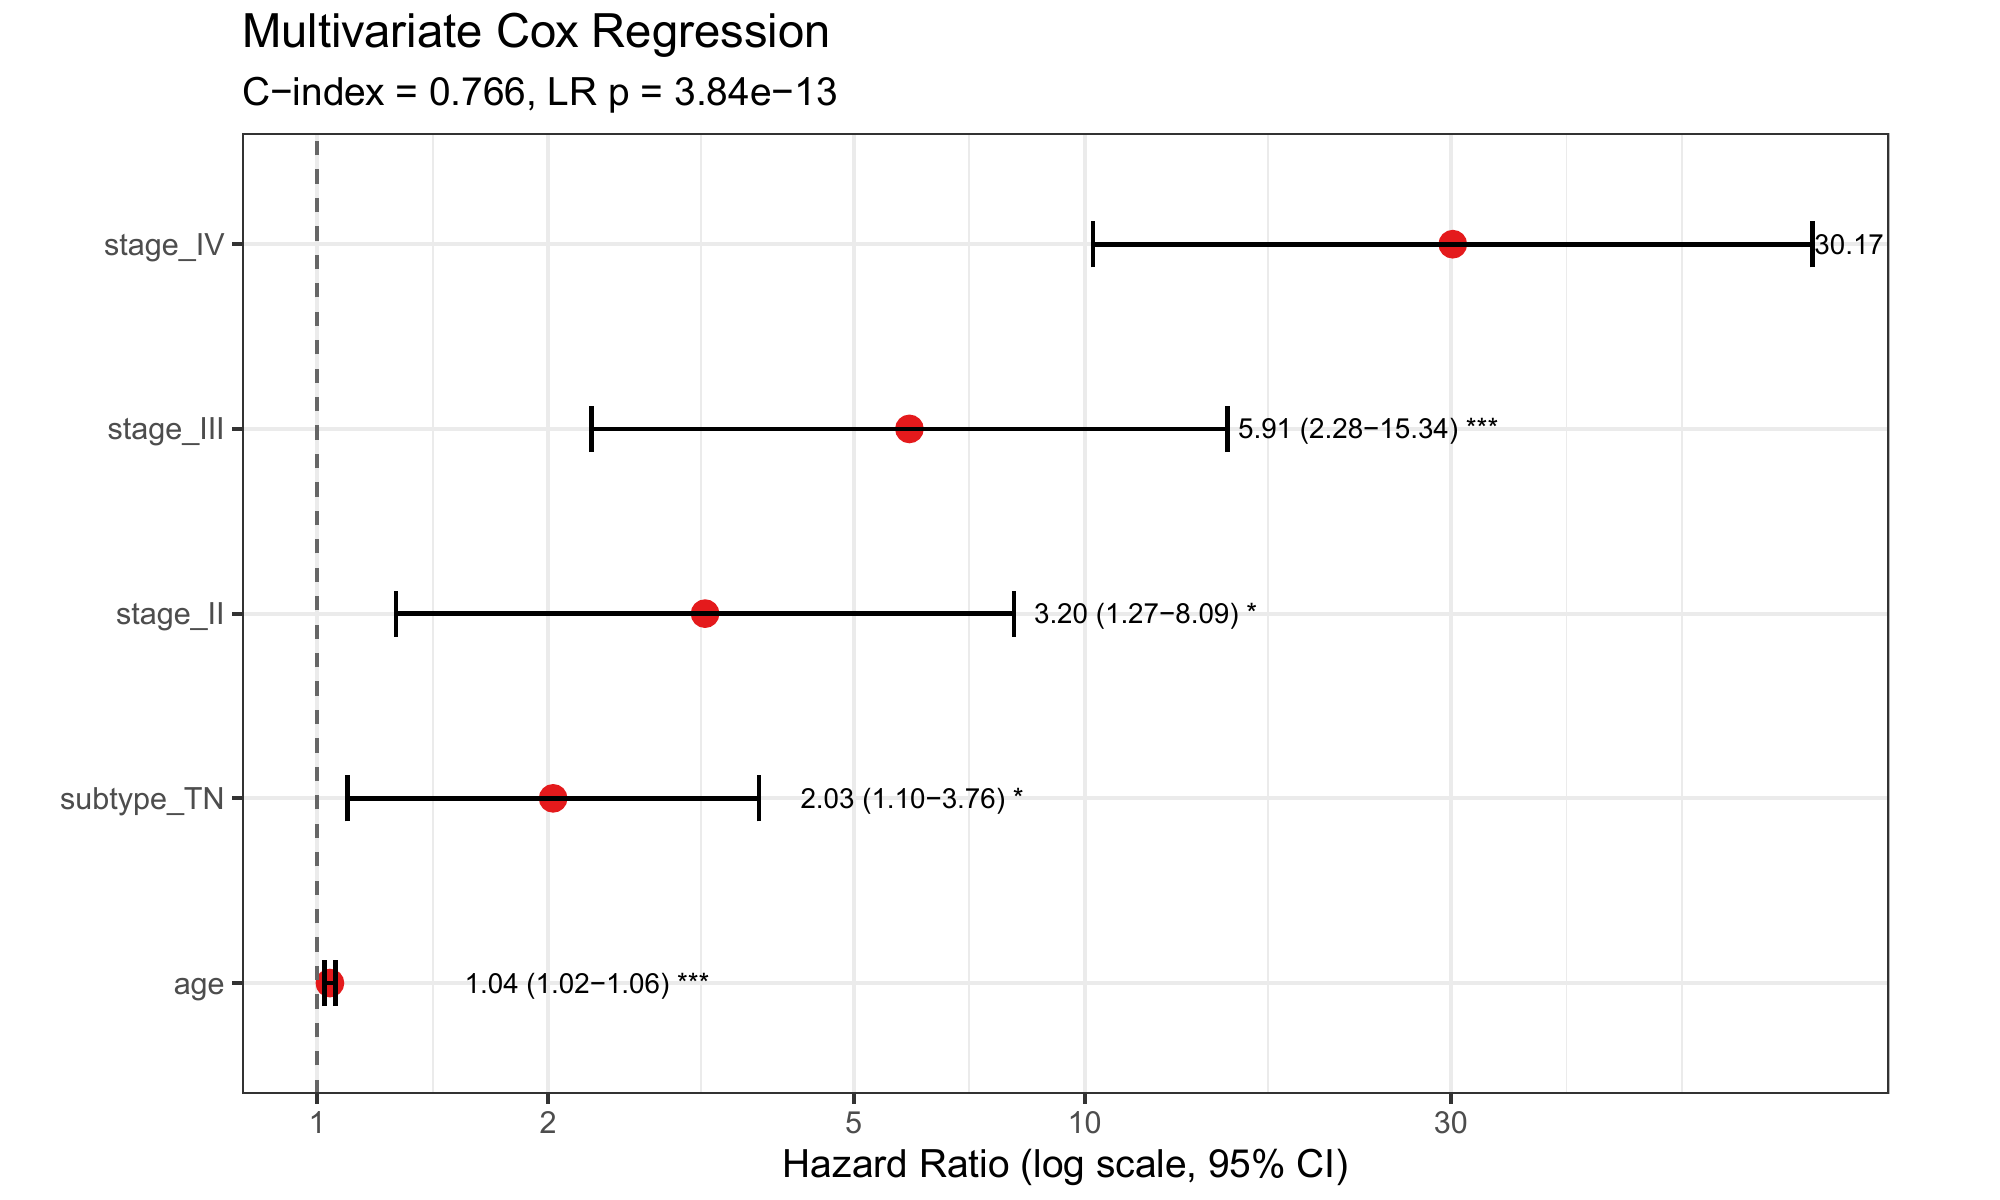
\includegraphics[width=0.85\textwidth]{figures/cox_forest_plot.png}
\caption{多变量Cox回归森林图}
\end{figure}

LASSO-Cox预后基因标记筛选出3个预后相关基因，按中位风险得分将患者分为高风险组和低风险组。

\begin{figure}[H]
\centering
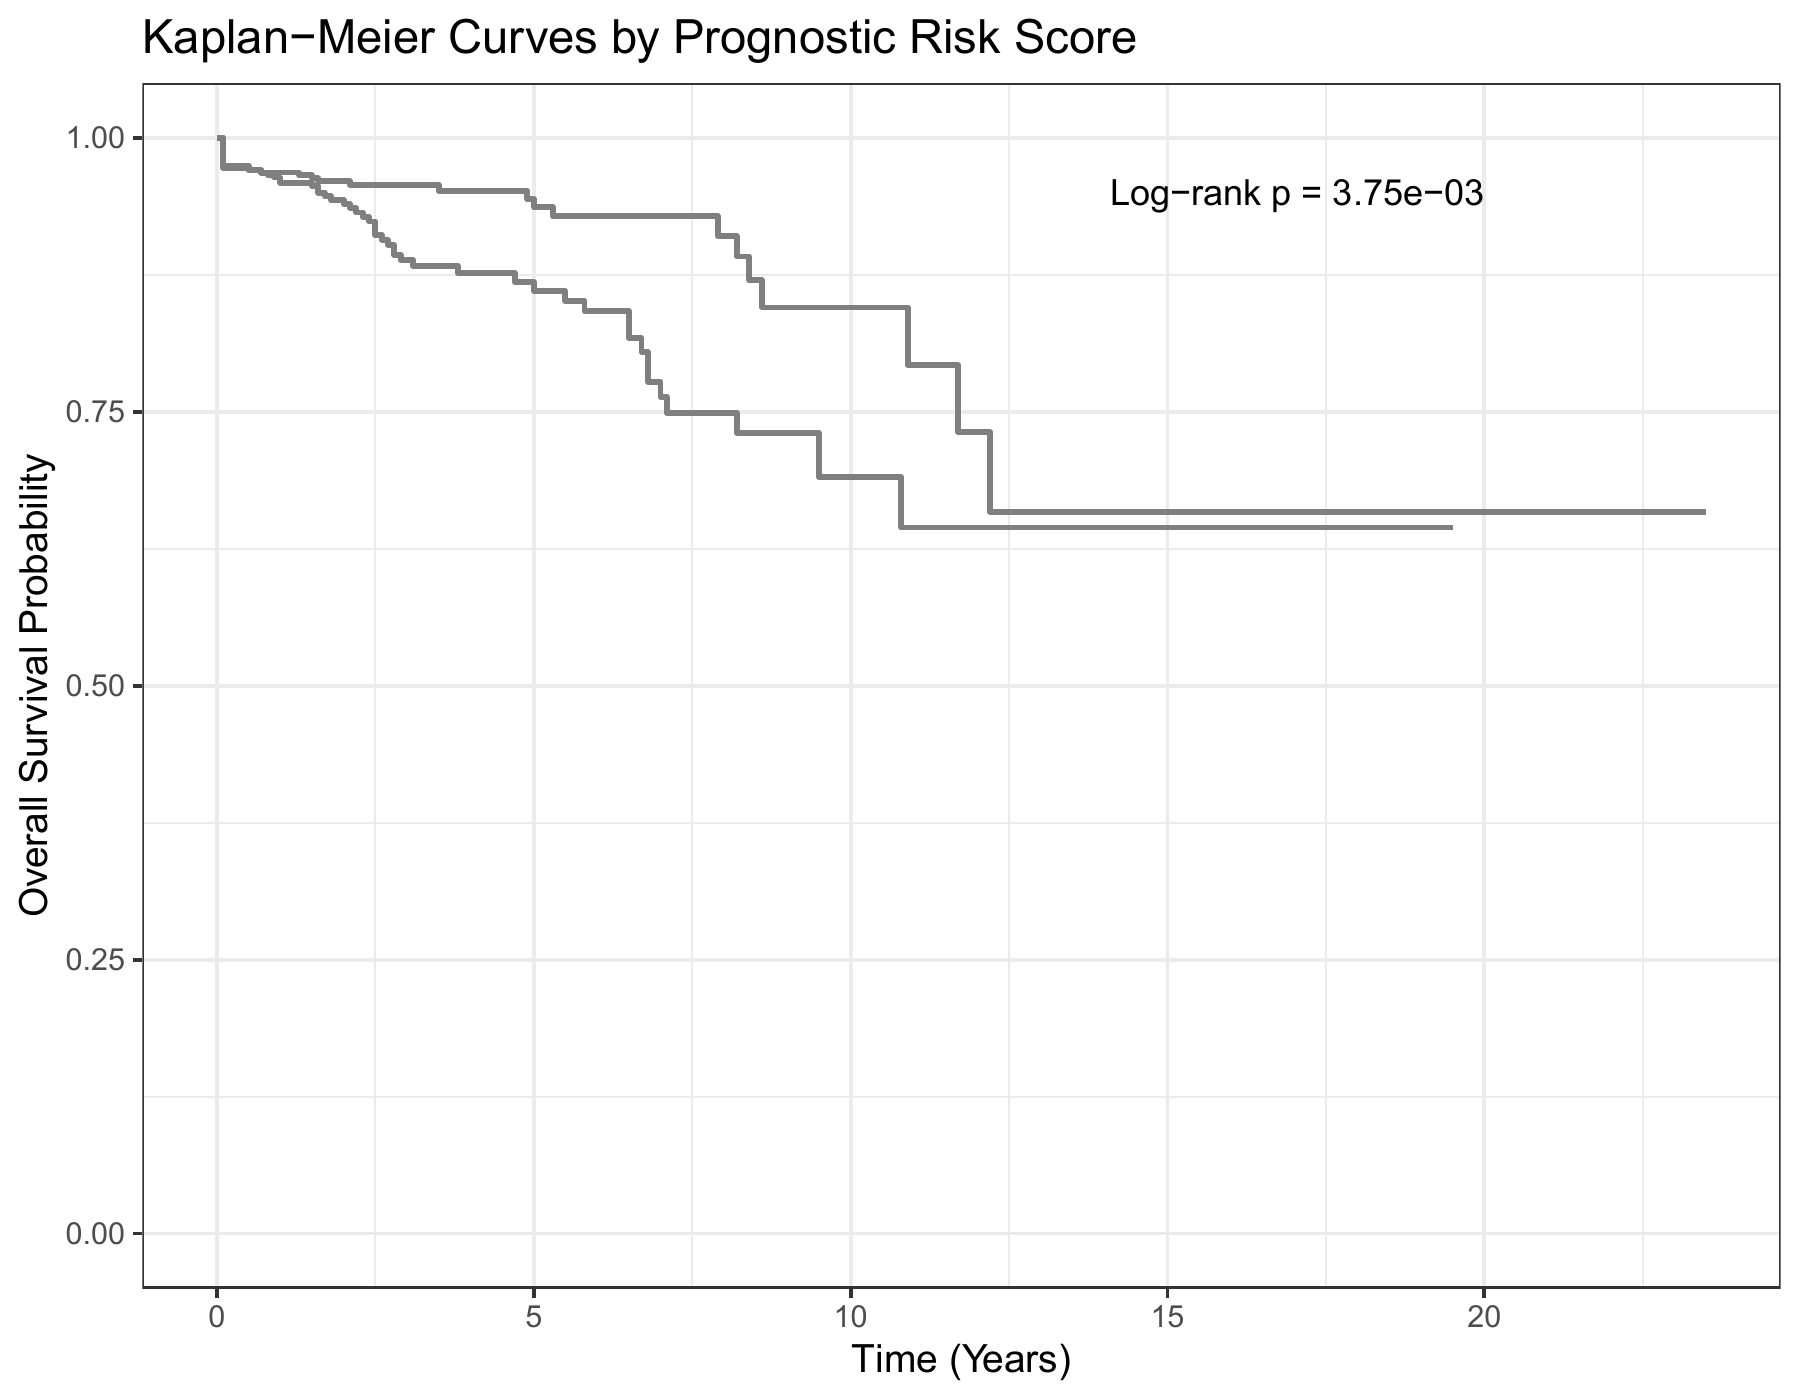
\includegraphics[width=0.85\textwidth]{figures/km_curves_signature.png}
\caption{LASSO-Cox预后基因标记风险分组KM曲线}
\end{figure}

% ===== 4 讨论 =====
\section{讨论}

本研究构建了覆盖差异表达分析、机器学习分类、聚类分析、WGCNA共表达网络和生存分析的完整数据挖掘流程。DESeq2鉴定6,768个差异表达基因，上调基因富集于细胞周期通路，与乳腺癌增殖活跃特征一致。LASSO分类器以较少特征基因实现了75.8\%的准确率，验证了亚型间转录组差异的稀疏性。PCA和K-means分析一致表明ER状态是BRCA转录组结构的最强驱动因素。WGCNA识别了与临床特征显著相关的共表达模块，枢纽基因是潜在的生物标志物候选。Cox回归证实病理分期为最强预后因子，Stage IV风险比高达29.82。

本研究存在以下局限性：（1）仅使用mRNA转录组数据，未纳入miRNA、DNA甲基化等多组学；（2）生存事件率较低（7.9\%），限制了预后模型的统计功效；（3）分类模型超参数未系统调优。未来方向包括多组学整合分析、独立队列外部验证、枢纽基因功能实验验证和单细胞测序解析。

% ===== 5 结论 =====
\section{结论}

本研究以TCGA-BRCA数据为基础，运用多种数据挖掘方法系统分析乳腺癌分子特征，主要结论如下：

（1）DESeq2差异表达分析鉴定6,768个显著差异基因，上调基因集中于细胞周期和DNA复制通路。

（2）Random Forest和LASSO分类器均达到75.8\%准确率，LASSO通过L1正则化实现了特征稀疏压缩。

（3）PCA（PC1=15.3\%）和K-means（K=2最优）表明ER状态是BRCA转录组的最强驱动因素。

（4）WGCNA识别9个共表达模块，枢纽基因模块隶属度最高达0.966。

（5）Cox回归C-index=0.767，病理分期为最强预后因子（Stage IV HR=29.82）。

% ===== 参考文献 =====
\newpage
\begin{center}
\textbf{参考文献}
\end{center}

\begin{thebibliography}{99}
\bibitem{sung2024} Sung H, Ferlay J, Siegel R L, et al. Global cancer statistics 2022: GLOBOCAN estimates of incidence and mortality worldwide for 36 cancers in 185 countries[J]. CA: A Cancer Journal for Clinicians, 2024, 74(3): 229-263.
\bibitem{hanahan2011} Hanahan D, Weinberg R A. Hallmarks of cancer: the next generation[J]. Cell, 2011, 144(5): 646-674.
\bibitem{tcga2012} Cancer Genome Atlas Network. Comprehensive molecular portraits of human breast tumours[J]. Nature, 2012, 490(7418): 61-70.
\bibitem{perou2000} Perou C M, Sorlie T, Eisen M B, et al. Molecular portraits of human breast tumours[J]. Nature, 2000, 406(6797): 747-752.
\bibitem{love2014} Love M I, Huber W, Anders S. Moderated estimation of fold change and dispersion for RNA-seq data with DESeq2[J]. Genome Biology, 2014, 15(12): 550.
\bibitem{langfelder2008} Langfelder P, Horvath S. WGCNA: an R package for weighted correlation network analysis[J]. BMC Bioinformatics, 2008, 9: 559.
\bibitem{simon2011} Simon N, Friedman J, Hastie T, et al. Regularization paths for Cox's proportional hazards model via coordinate descent[J]. Journal of Statistical Software, 2011, 39(5): 1-13.
\bibitem{kolberg2023} Kolberg L, Raudvere U, Kuzmin I, et al. g:Profiler---interoperable web service for functional enrichment analysis and gene identifier mapping (2023 update)[J]. Nucleic Acids Research, 2023, 51(W1): W207-W212.
\bibitem{wilkerson2010} Wilkerson M D, Hayes D N. ConsensusClusterPlus: a class discovery tool with confidence assessments and item tracking[J]. Bioinformatics, 2010, 26(12): 1572-1573.
\bibitem{colaprico2016} Colaprico A, Silva T C, Olsen C, et al. TCGAbiolinks: an R/Bioconductor package for integrative analysis of TCGA data[J]. Nucleic Acids Research, 2016, 44(8): e71.
\bibitem{mayakoda2018} Mayakonda A, Lin D C, Assenov Y, et al. Maftools: efficient and comprehensive analysis of somatic variants in cancer[J]. Genome Research, 2018, 28(11): 1747-1756.
\bibitem{friedman2010} Friedman J, Hastie T, Tibshirani R. Regularization paths for generalized linear models via coordinate descent[J]. Journal of Statistical Software, 2010, 33(1): 1-22.
\bibitem{breiman2001} Breiman L. Random forests[J]. Machine Learning, 2001, 45(1): 5-32.
\bibitem{chen2016} Chen T, Guestrin C. XGBoost: a scalable tree boosting system[C]. Proceedings of the 22nd ACM SIGKDD, 2016: 785-794.
\bibitem{therneau2000} Therneau T M, Grambsch P M. Modeling survival data: extending the Cox model[M]. New York: Springer, 2000.
\bibitem{tibshirani1996} Tibshirani R. Regression shrinkage and selection via the lasso[J]. Journal of the Royal Statistical Society: Series B, 1996, 58(1): 267-288.
\end{thebibliography}

% ===== 附录A =====
\newpage
\begin{center}
\textbf{附录A\quad 核心R代码}
\end{center}

\subsection{数据预处理}

\begin{lstlisting}[caption={加载数据与样本分类}]
load("brca_exp.Rdata")
load("brca_clinical.Rdata")
barcodes <- colnames(brca)
sample_code <- substr(barcodes, 14, 15)
tumor_idx  <- which(sample_code == "01")
normal_idx <- which(sample_code == "11")
counts_tumor  <- brca[, tumor_idx]
counts_normal <- brca[, normal_idx]
keep <- rowSums(counts_tumor >= 10) >=
  ceiling(ncol(counts_tumor) * 0.1)
counts_tumor <- counts_tumor[keep, ]
\end{lstlisting}

\begin{lstlisting}[caption={基因标识符映射与TPM标准化}]
library(org.Hs.eg.db)
gene_map <- AnnotationDbi::select(org.Hs.eg.db,
  keys = ensembl_clean,
  columns = "SYMBOL", keytype = "ENSEMBL")
counts_to_tpm <- function(counts, gene_lengths) {
  rpk <- counts / (gene_lengths / 1000)
  sweep(rpk, 2, colSums(rpk) / 1e6, "/")
}
tpm_tumor <- counts_to_tpm(counts_tumor, gene_length_vec)
\end{lstlisting}

\subsection{差异表达分析}

\begin{lstlisting}[caption={DESeq2差异表达分析}]
library(DESeq2)
dds <- DESeqDataSetFromMatrix(
  countData = round(counts_combined),
  colData   = col_data,
  design    = ~ condition)
keep <- rowSums(counts(dds) >= 10) >=
  min(10, ncol(dds) / 10)
dds <- dds[keep, ]
dds <- DESeq(dds)
res <- results(dds,
  contrast = c("condition", "Tumor", "Normal"),
  alpha = 0.05)
deg <- subset(as.data.frame(res),
  padj < 0.05 & abs(log2FoldChange) > 1)
\end{lstlisting}

\subsection{机器学习分类}

\begin{lstlisting}[caption={Random Forest与LASSO分类}]
library(caret)
library(randomForest)
library(glmnet)
log_tpm <- log2(tpm_sub + 1)
top500 <- names(sort(apply(log_tpm, 1, var),
  decreasing = TRUE))[1:500]
X <- t(log_tpm[top500, ])
set.seed(42)
idx <- createDataPartition(y, p = 0.7, list = FALSE)
X_train <- X[idx, ]; X_test <- X[-idx, ]
y_train <- y[idx];    y_test <- y[-idx, ]
rf <- randomForest(x = X_train, y = y_train,
  ntree = 500, importance = TRUE)
cv_lasso <- cv.glmnet(x = X_train, y = y_train,
  family = "multinomial", alpha = 1, nfolds = 5)
\end{lstlisting}

\subsection{聚类分析}

\begin{lstlisting}[caption={PCA、t-SNE与K-means}]
pca <- prcomp(t(log_tpm_top),
  center = TRUE, scale. = TRUE)
library(Rtsne)
tsne <- Rtsne(t(log_tpm_top),
  perplexity = 30, max_iter = 1000)
set.seed(42)
for (k in 2:10) {
  km <- kmeans(t(log_tpm_top), centers = k, nstart = 25)
  sil[k] <- mean(cluster::silhouette(
    km$cluster, dist(t(log_tpm_top)))[, 3])
}
\end{lstlisting}

\subsection{WGCNA共表达网络分析}

\begin{lstlisting}[caption={WGCNA网络构建}]
library(WGCNA)
sft <- pickSoftThreshold(datExpr,
  powerVector = 1:20, networkType = "signed")
net <- blockwiseModules(datExpr,
  power = soft_power, TOMType = "signed",
  minModuleSize = 30, mergeCutHeight = 0.25)
module_colors <- labels2colors(net$colors)
MEs <- net$MEs
module_trait_cor <- cor(MEs, traits, use = "p")
\end{lstlisting}

\subsection{生存分析}

\begin{lstlisting}[caption={KM曲线与Cox回归}]
library(survival)
library(survminer)
fit <- survfit(Surv(os_time_years, os_status)
  ~ stage_simple, data = clinical)
cox_model <- coxph(Surv(os_time, os_status) ~
  age + stage_II + stage_III + stage_IV +
  subtype_TN, data = cox_data)
cv_cox <- cv.glmnet(x = X,
  y = Surv(time, status),
  family = "cox", alpha = 1, nfolds = 5)
\end{lstlisting}

\end{document}
